\documentclass[conference]{IEEEtran}
\IEEEoverridecommandlockouts
\usepackage[T1]{fontenc}
\usepackage{microtype}
\usepackage{amsmath,amssymb,amsthm,bm}
\usepackage{booktabs,graphicx,xcolor,array,enumitem}
\usepackage[ruled,vlined,linesnumbered]{algorithm2e}
\usepackage{dblfloatfix}
\usepackage[colorlinks=true,linkcolor=blue!50!black,citecolor=blue!50!black,urlcolor=blue!50!black]{hyperref}

% Every number in this report is a macro written by experiments/make_figures.py from the files in results/.
% AUTO-GENERATED by experiments/make_figures.py from results/*.json -- do not edit by hand.
\newcommand{\AgreeEpsEoneBar}{86}
\newcommand{\AgreeEpsEoneSeats}{71}
\newcommand{\AgreeEpsEtwoBar}{86}
\newcommand{\AgreeEpsEtwoSeats}{72}
\newcommand{\AgreeEpsEzeroBar}{74}
\newcommand{\AgreeEpsEzeroSeats}{82}
\newcommand{\AgreeExpEoneBar}{94}
\newcommand{\AgreeExpEoneSeats}{81}
\newcommand{\AgreeExpEtwoBar}{93}
\newcommand{\AgreeExpEtwoSeats}{84}
\newcommand{\AgreeExpEzeroBar}{51}
\newcommand{\AgreeExpEzeroSeats}{93}
\newcommand{\AgreeEzeroBarMax}{74}
\newcommand{\AgreeEzeroBarMin}{51}
\newcommand{\AgreeMbEoneBar}{100}
\newcommand{\AgreeMbEoneSeats}{100}
\newcommand{\AgreeMbEtwoBar}{100}
\newcommand{\AgreeMbEtwoSeats}{100}
\newcommand{\AgreeMbEzeroBar}{56}
\newcommand{\AgreeMbEzeroSeats}{96}
\newcommand{\AgreeMidEpsEoneBar}{71}
\newcommand{\AgreeMidEpsEoneSeats}{57}
\newcommand{\AgreeMidEpsEtwoBar}{72}
\newcommand{\AgreeMidEpsEtwoSeats}{59}
\newcommand{\AgreeMidEpsEzeroBar}{72}
\newcommand{\AgreeMidEpsEzeroSeats}{77}
\newcommand{\AgreeMidExpEoneBar}{79}
\newcommand{\AgreeMidExpEoneSeats}{61}
\newcommand{\AgreeMidExpEtwoBar}{78}
\newcommand{\AgreeMidExpEtwoSeats}{61}
\newcommand{\AgreeMidExpEzeroBar}{55}
\newcommand{\AgreeMidExpEzeroSeats}{81}
\newcommand{\AgreeMidMbEoneBar}{99}
\newcommand{\AgreeMidMbEoneSeats}{93}
\newcommand{\AgreeMidMbEtwoBar}{99}
\newcommand{\AgreeMidMbEtwoSeats}{93}
\newcommand{\AgreeMidMbEzeroBar}{54}
\newcommand{\AgreeMidMbEzeroSeats}{91}
\newcommand{\AgreeMidMuEoneBar}{100}
\newcommand{\AgreeMidMuEoneSeats}{98}
\newcommand{\AgreeMidMuEtwoBar}{100}
\newcommand{\AgreeMidMuEtwoSeats}{96}
\newcommand{\AgreeMidMuEzeroBar}{52}
\newcommand{\AgreeMidMuEzeroSeats}{90}
\newcommand{\AgreeMidTsEoneBar}{92}
\newcommand{\AgreeMidTsEoneSeats}{71}
\newcommand{\AgreeMidTsEtwoBar}{91}
\newcommand{\AgreeMidTsEtwoSeats}{67}
\newcommand{\AgreeMidTsEzeroBar}{61}
\newcommand{\AgreeMidTsEzeroSeats}{92}
\newcommand{\AgreeMidUcbEoneBar}{93}
\newcommand{\AgreeMidUcbEoneSeats}{82}
\newcommand{\AgreeMidUcbEtwoBar}{95}
\newcommand{\AgreeMidUcbEtwoSeats}{80}
\newcommand{\AgreeMidUcbEzeroBar}{54}
\newcommand{\AgreeMidUcbEzeroSeats}{91}
\newcommand{\AgreeMuEoneBar}{100}
\newcommand{\AgreeMuEoneSeats}{100}
\newcommand{\AgreeMuEtwoBar}{100}
\newcommand{\AgreeMuEtwoSeats}{100}
\newcommand{\AgreeMuEzeroBar}{53}
\newcommand{\AgreeMuEzeroSeats}{96}
\newcommand{\AgreePooledEps}{78}
\newcommand{\AgreePooledExp}{83}
\newcommand{\AgreePooledMb}{92}
\newcommand{\AgreePooledMu}{92}
\newcommand{\AgreePooledTs}{91}
\newcommand{\AgreePooledUcb}{90}
\newcommand{\AgreeTsEoneBar}{99}
\newcommand{\AgreeTsEoneSeats}{92}
\newcommand{\AgreeTsEtwoBar}{99}
\newcommand{\AgreeTsEtwoSeats}{94}
\newcommand{\AgreeTsEzeroBar}{70}
\newcommand{\AgreeTsEzeroSeats}{93}
\newcommand{\AgreeUcbEoneBar}{99}
\newcommand{\AgreeUcbEoneSeats}{93}
\newcommand{\AgreeUcbEtwoBar}{99}
\newcommand{\AgreeUcbEtwoSeats}{94}
\newcommand{\AgreeUcbEzeroBar}{56}
\newcommand{\AgreeUcbEzeroSeats}{96}
\newcommand{\AstarGridBarAvg}{0.025}
\newcommand{\AstarGridBarStrong}{0.025}
\newcommand{\AstarGridBarWeak}{0.025}
\newcommand{\AstarGridSeatsAvg}{0.325--0.35}
\newcommand{\AstarGridSeatsStrong}{0.375--0.4}
\newcommand{\AstarGridSeatsWeak}{0.125}
\newcommand{\AstarLocalBarAvg}{0.01}
\newcommand{\AstarLocalBarStrong}{0.01}
\newcommand{\AstarLocalBarWeak}{0.01}
\newcommand{\AstarLocalSeatsAvg}{0.32}
\newcommand{\AstarLocalSeatsStrong}{0.38}
\newcommand{\AstarLocalSeatsWeak}{0.10}
\newcommand{\BarSeatsHigher}{12}
\newcommand{\BarSeatsNotSigLearners}{Leak-aware UCB, Model-based UCB}
\newcommand{\BarSeatsSig}{8}
\newcommand{\BarSeatsTests}{12}
\newcommand{\BaseEqBelowRandomBar}{yes}
\newcommand{\BaseLearnBelowWelfare}{0}
\newcommand{\BaseVEqBar}{0.771}
\newcommand{\BaseVEqSeats}{0.645}
\newcommand{\BaseVEveryBar}{0.771}
\newcommand{\BaseVEverySeats}{0.614}
\newcommand{\BaseVLearnMinBar}{0.771}
\newcommand{\BaseVLearnMinSeats}{0.638}
\newcommand{\BaseVNobodyBar}{0.894}
\newcommand{\BaseVNobodySeats}{0.657}
\newcommand{\BaseVRandomBar}{0.833}
\newcommand{\BaseVRandomSeats}{0.631}
\newcommand{\BaseWEqBar}{3.317}
\newcommand{\BaseWEqSeats}{2.798}
\newcommand{\BaseWEveryBar}{3.317}
\newcommand{\BaseWEverySeats}{2.794}
\newcommand{\BaseWLearnMinBar}{3.256}
\newcommand{\BaseWLearnMinSeats}{2.797}
\newcommand{\BaseWNobodyBar}{2.799}
\newcommand{\BaseWNobodySeats}{2.800}
\newcommand{\BaseWRandomBar}{3.067}
\newcommand{\BaseWRandomSeats}{2.797}
\newcommand{\CceCrossMaxDiff}{$<10^{-12}$}
\newcommand{\CceCrossRows}{212}
\newcommand{\CceEETot}{212}
\newcommand{\CceEtwoAboveMax}{0}
\newcommand{\CceEtwoAboveN}{0}
\newcommand{\CceEtwoBelowMax}{0}
\newcommand{\CceEtwoBelowN}{0}
\newcommand{\CceEtwoEqual}{106}
\newcommand{\CceEtwoMultiBne}{0}
\newcommand{\CceEtwoSingle}{106}
\newcommand{\CceEtwoTot}{106}
\newcommand{\CceEtwoWide}{0}
\newcommand{\CceEtwoWideMulti}{0}
\newcommand{\CceExHi}{99}
\newcommand{\CceExLo}{66}
\newcommand{\CceExN}{4}
\newcommand{\CceExPure}{67}
\newcommand{\CceEzeroAboveMax}{33}
\newcommand{\CceEzeroAboveN}{48}
\newcommand{\CceEzeroBarStarPure}{80}
\newcommand{\CceEzeroBarStarTop}{99.8}
\newcommand{\CceEzeroBarTwoPure}{67}
\newcommand{\CceEzeroBarTwoTop}{99.6}
\newcommand{\CceEzeroBelowMax}{8}
\newcommand{\CceEzeroBelowN}{45}
\newcommand{\CceEzeroEqual}{58}
\newcommand{\CceEzeroMultiBne}{49}
\newcommand{\CceEzeroPairsEqual}{42}
\newcommand{\CceEzeroPairsTot}{42}
\newcommand{\CceEzeroSingle}{55}
\newcommand{\CceEzeroTot}{106}
\newcommand{\CceEzeroWide}{48}
\newcommand{\CceEzeroWideMulti}{46}
\newcommand{\CceMaxWidth}{0.417}
\newcommand{\CceMaxWidthEone}{0}
\newcommand{\CceMaxWidthEtwo}{0}
\newcommand{\CceMaxWidthEzero}{42}
\newcommand{\CceSingle}{267}
\newcommand{\CceSingleEone}{106}
\newcommand{\CceSingleEtwo}{106}
\newcommand{\CceSingleEzero}{55}
\newcommand{\CceTot}{318}
\newcommand{\CceTotEone}{106}
\newcommand{\CceTotEtwo}{106}
\newcommand{\CceTotEzero}{106}
\newcommand{\CceWiderEone}{0}
\newcommand{\CceWiderEtwo}{0}
\newcommand{\CceWiderEzero}{48}
\newcommand{\ChkDevPos}{0}
\newcommand{\ChkDevTot}{684}
\newcommand{\ChkDiya}{0.7088}
\newcommand{\ChkKabir}{0.7085}
\newcommand{\ChkOvertake}{0.9157}
\newcommand{\ChkPropThreeWorst}{2.2}
\newcommand{\ChkSpread}{0.29}
\newcommand{\ClanAlphaEffFull}{0.41}
\newcommand{\ClanBetaFull}{0.35}
\newcommand{\ClanMonotoneBar}{yes}
\newcommand{\ClanMonotoneSeats}{yes}
\newcommand{\ClanShareMaxBar}{100}
\newcommand{\ClanShareMaxSeats}{100}
\newcommand{\ClanShareMinBar}{100}
\newcommand{\ClanShareMinSeats}{33}
\newcommand{\CompBarAllShare}{19}
\newcommand{\CompGrid}{21}
\newcommand{\CompGridPos}{20}
\newcommand{\CompSeatsAllShare}{0}
\newcommand{\CompSeatsNoShare}{21}
\newcommand{\CrossQBarBetterFrom}{9}
\newcommand{\CrossQBarWorseUpTo}{6}
\newcommand{\DomOpenOutsideEzero}{1}
\newcommand{\DomOpenWhere}{two friend groups, E1, fixed seats, $\alpha=0.1$}
\newcommand{\DomPairsEoneSolved}{42}
\newcommand{\DomPairsEoneTot}{42}
\newcommand{\DomPairsEtwoSolved}{42}
\newcommand{\DomPairsEtwoTot}{42}
\newcommand{\DomPairsEzeroSolved}{39}
\newcommand{\DomPairsEzeroTot}{42}
\newcommand{\DomPairsSolved}{123}
\newcommand{\DomPairsTot}{126}
\newcommand{\DomSolved}{311}
\newcommand{\DomStarEoneSolved}{42}
\newcommand{\DomStarEoneTot}{42}
\newcommand{\DomStarEtwoSolved}{42}
\newcommand{\DomStarEtwoTot}{42}
\newcommand{\DomStarEzeroSolved}{12}
\newcommand{\DomStarEzeroTot}{42}
\newcommand{\DomStarSolved}{96}
\newcommand{\DomStarTot}{126}
\newcommand{\DomTot}{378}
\newcommand{\DomTwoGroupsEoneSolved}{41}
\newcommand{\DomTwoGroupsEoneTot}{42}
\newcommand{\DomTwoGroupsEtwoSolved}{42}
\newcommand{\DomTwoGroupsEtwoTot}{42}
\newcommand{\DomTwoGroupsEzeroSolved}{9}
\newcommand{\DomTwoGroupsEzeroTot}{42}
\newcommand{\DomTwoGroupsSolved}{92}
\newcommand{\DomTwoGroupsTot}{126}
\newcommand{\EllBarAvg}{0.00}
\newcommand{\EllBarStrong}{0.00}
\newcommand{\EllBarWeak}{0.00}
\newcommand{\EllSeatsAvg}{1.49}
\newcommand{\EllSeatsStrong}{1.60}
\newcommand{\EllSeatsWeak}{0.38}
\newcommand{\EpsBneEzero}{62}
\newcommand{\EpsBneGames}{378}
\newcommand{\EpsBneHeadBar}{1}
\newcommand{\EpsBneHeadSeats}{1}
\newcommand{\EpsBneLowAlpha}{17}
\newcommand{\EpsBneMulti}{117}
\newcommand{\EpsBneStep}{38}
\newcommand{\EpsBneStepMax}{64}
\newcommand{\EtwoBiasControlMax}{0.06}
\newcommand{\EtwoBiasDays}{4\,million}
\newcommand{\EtwoBiasGap}{0.36}
\newcommand{\EtwoBiasMax}{0.08}
\newcommand{\EtwoBiasOverGap}{22}
\newcommand{\EtwoBiasSe}{0.03}
\newcommand{\ExactEqEpsEoneBar}{3}
\newcommand{\ExactEqEpsEoneSeats}{0}
\newcommand{\ExactEqEpsEtwoBar}{10}
\newcommand{\ExactEqEpsEtwoSeats}{0}
\newcommand{\ExactEqEpsEzeroBar}{0}
\newcommand{\ExactEqEpsEzeroSeats}{13}
\newcommand{\ExactEqExpEoneBar}{30}
\newcommand{\ExactEqExpEoneSeats}{3}
\newcommand{\ExactEqExpEtwoBar}{30}
\newcommand{\ExactEqExpEtwoSeats}{3}
\newcommand{\ExactEqExpEzeroBar}{0}
\newcommand{\ExactEqExpEzeroSeats}{20}
\newcommand{\ExactEqMbEoneBar}{100}
\newcommand{\ExactEqMbEoneSeats}{97}
\newcommand{\ExactEqMbEtwoBar}{100}
\newcommand{\ExactEqMbEtwoSeats}{100}
\newcommand{\ExactEqMbEzeroBar}{0}
\newcommand{\ExactEqMbEzeroSeats}{70}
\newcommand{\ExactEqMuEoneBar}{100}
\newcommand{\ExactEqMuEoneSeats}{100}
\newcommand{\ExactEqMuEtwoBar}{100}
\newcommand{\ExactEqMuEtwoSeats}{93}
\newcommand{\ExactEqMuEzeroBar}{0}
\newcommand{\ExactEqMuEzeroSeats}{63}
\newcommand{\ExactEqTsEoneBar}{87}
\newcommand{\ExactEqTsEoneSeats}{33}
\newcommand{\ExactEqTsEtwoBar}{83}
\newcommand{\ExactEqTsEtwoSeats}{27}
\newcommand{\ExactEqTsEzeroBar}{0}
\newcommand{\ExactEqTsEzeroSeats}{37}
\newcommand{\ExactEqUcbEoneBar}{87}
\newcommand{\ExactEqUcbEoneSeats}{40}
\newcommand{\ExactEqUcbEtwoBar}{93}
\newcommand{\ExactEqUcbEtwoSeats}{50}
\newcommand{\ExactEqUcbEzeroBar}{0}
\newcommand{\ExactEqUcbEzeroSeats}{70}
\newcommand{\ExactEzeroBarMax}{0}
\newcommand{\ExpAvgHardest}{yes}
\newcommand{\ExpCostMatchPct}{6}
\newcommand{\ExpMistakeGapEpsBar}{1.00}
\newcommand{\ExpMistakeGapEpsSeats}{1.01}
\newcommand{\ExpPoolFourEoneBar}{86}
\newcommand{\ExpPoolFourEoneSeats}{34}
\newcommand{\ExpPoolOf}{4}
\newcommand{\ExpPoolTwoEoneBar}{81}
\newcommand{\ExpPoolTwoEoneSeats}{25}
\newcommand{\ExpPoolWins}{4}
\newcommand{\ExpRhoTs}{0.70}
\newcommand{\ExpRhoUcb}{0.80}
\newcommand{\ExpSdAvg}{0.30}
\newcommand{\ExpSdStrong}{0.31}
\newcommand{\ExpSdWeak}{0.15}
\newcommand{\ExpSnrAvg}{2{,}934}
\newcommand{\ExpSnrStrong}{1{,}730}
\newcommand{\ExpSnrWeak}{1{,}474}
\newcommand{\ExpWrongEpsBar}{23}
\newcommand{\ExpWrongEpsSeats}{37}
\newcommand{\ExpWrongExpBar}{51}
\newcommand{\ExpWrongExpSeats}{57}
\newcommand{\ExpWrongMuBar}{9}
\newcommand{\ExpWrongMuSeats}{41}
\newcommand{\ExpWrongTsBar}{23}
\newcommand{\ExpWrongTsSeats}{41}
\newcommand{\ExpWrongUcbBar}{48}
\newcommand{\ExpWrongUcbSeats}{56}
\newcommand{\ExplEpsEoneBar}{1.10}
\newcommand{\ExplEpsEoneSeats}{0.80}
\newcommand{\ExplEpsEtwoBar}{1.03}
\newcommand{\ExplEpsEtwoSeats}{0.79}
\newcommand{\ExplEpsEzeroBar}{0.10}
\newcommand{\ExplEpsEzeroSeats}{1.25}
\newcommand{\ExplExpEoneBar}{0.81}
\newcommand{\ExplExpEoneSeats}{0.75}
\newcommand{\ExplExpEtwoBar}{0.79}
\newcommand{\ExplExpEtwoSeats}{0.77}
\newcommand{\ExplExpEzeroBar}{0.10}
\newcommand{\ExplExpEzeroSeats}{0.66}
\newcommand{\ExplEzeroBarMax}{0.10}
\newcommand{\ExplEzeroBarMin}{0.10}
\newcommand{\ExplMbEoneBar}{0.00}
\newcommand{\ExplMbEoneSeats}{0.02}
\newcommand{\ExplMbEtwoBar}{0.00}
\newcommand{\ExplMbEtwoSeats}{0.00}
\newcommand{\ExplMbEzeroBar}{0.10}
\newcommand{\ExplMbEzeroSeats}{0.17}
\newcommand{\ExplMuEoneBar}{0.00}
\newcommand{\ExplMuEoneSeats}{0.00}
\newcommand{\ExplMuEtwoBar}{0.00}
\newcommand{\ExplMuEtwoSeats}{0.04}
\newcommand{\ExplMuEzeroBar}{0.10}
\newcommand{\ExplMuEzeroSeats}{0.27}
\newcommand{\ExplTsEoneBar}{0.14}
\newcommand{\ExplTsEoneSeats}{0.42}
\newcommand{\ExplTsEtwoBar}{0.16}
\newcommand{\ExplTsEtwoSeats}{0.48}
\newcommand{\ExplTsEzeroBar}{0.10}
\newcommand{\ExplTsEzeroSeats}{0.33}
\newcommand{\ExplUcbEoneBar}{0.14}
\newcommand{\ExplUcbEoneSeats}{0.36}
\newcommand{\ExplUcbEtwoBar}{0.07}
\newcommand{\ExplUcbEtwoSeats}{0.31}
\newcommand{\ExplUcbEzeroBar}{0.10}
\newcommand{\ExplUcbEzeroSeats}{0.17}
\newcommand{\EzmCHi}{0.02}
\newcommand{\EzmCLo}{0.0005}
\newcommand{\EzmCRatio}{40}
\newcommand{\EzmFallsBar}{yes}
\newcommand{\EzmFallsSeats}{yes}
\newcommand{\EzmPred}{yes}
\newcommand{\EzmRedundantBar}{100}
\newcommand{\EzmRedundantSeats}{107}
\newcommand{\EzmSeatsClosedFrom}{0.005}
\newcommand{\EzmWidthBarBase}{33}
\newcommand{\EzmWidthBarHi}{28}
\newcommand{\EzmWidthBarLo}{33}
\newcommand{\EzmWidthSeatsBase}{40}
\newcommand{\EzmWidthSeatsHi}{0}
\newcommand{\EzmWidthSeatsLo}{45}
\newcommand{\GainBarAvg}{6.7}
\newcommand{\GainBarStrong}{6.7}
\newcommand{\GainBarWeak}{6.7}
\newcommand{\GainSeatsAvg}{4.9}
\newcommand{\GainSeatsStrong}{4.5}
\newcommand{\GainSeatsWeak}{4.5}
\newcommand{\GapEpsEoneBar}{0.51}
\newcommand{\GapEpsEoneSeats}{0.44}
\newcommand{\GapEpsEtwoBar}{0.51}
\newcommand{\GapEpsEtwoSeats}{0.42}
\newcommand{\GapEpsEzeroBar}{0.21}
\newcommand{\GapEpsEzeroSeats}{0.48}
\newcommand{\GapExpEoneBar}{0.94}
\newcommand{\GapExpEoneSeats}{0.54}
\newcommand{\GapExpEtwoBar}{0.93}
\newcommand{\GapExpEtwoSeats}{0.52}
\newcommand{\GapExpEzeroBar}{1.55}
\newcommand{\GapExpEzeroSeats}{1.15}
\newcommand{\GapFallSetSig}{36}
\newcommand{\GapFallSetSigEonetwo}{24}
\newcommand{\GapFallSetTests}{36}
\newcommand{\GapFallSetTestsEonetwo}{24}
\newcommand{\GapFallSig}{6}
\newcommand{\GapFallTests}{6}
\newcommand{\GapFinalEps}{0.43}
\newcommand{\GapFinalExp}{0.94}
\newcommand{\GapFinalMax}{0.94}
\newcommand{\GapFinalMb}{0.60}
\newcommand{\GapFinalMin}{0.38}
\newcommand{\GapFinalMu}{0.44}
\newcommand{\GapFinalTs}{0.38}
\newcommand{\GapFinalUcb}{0.83}
\newcommand{\GapMbEoneBar}{0.16}
\newcommand{\GapMbEoneSeats}{0.52}
\newcommand{\GapMbEtwoBar}{0.24}
\newcommand{\GapMbEtwoSeats}{0.52}
\newcommand{\GapMbEzeroBar}{1.14}
\newcommand{\GapMbEzeroSeats}{1.01}
\newcommand{\GapMuEoneBar}{0.14}
\newcommand{\GapMuEoneSeats}{0.35}
\newcommand{\GapMuEtwoBar}{0.20}
\newcommand{\GapMuEtwoSeats}{0.37}
\newcommand{\GapMuEzeroBar}{0.83}
\newcommand{\GapMuEzeroSeats}{0.76}
\newcommand{\GapRatioEps}{0.52}
\newcommand{\GapRatioExp}{0.73}
\newcommand{\GapRatioMax}{0.73}
\newcommand{\GapRatioMb}{0.53}
\newcommand{\GapRatioMin}{0.42}
\newcommand{\GapRatioMu}{0.42}
\newcommand{\GapRatioTs}{0.45}
\newcommand{\GapRatioUcb}{0.73}
\newcommand{\GapTenKEps}{0.89}
\newcommand{\GapTenKExp}{1.67}
\newcommand{\GapTenKMb}{1.28}
\newcommand{\GapTenKMu}{1.17}
\newcommand{\GapTenKTs}{1.04}
\newcommand{\GapTenKUcb}{1.42}
\newcommand{\GapTsEoneBar}{0.46}
\newcommand{\GapTsEoneSeats}{0.39}
\newcommand{\GapTsEtwoBar}{0.48}
\newcommand{\GapTsEtwoSeats}{0.40}
\newcommand{\GapTsEzeroBar}{0.24}
\newcommand{\GapTsEzeroSeats}{0.33}
\newcommand{\GapUcbEoneBar}{0.90}
\newcommand{\GapUcbEoneSeats}{0.52}
\newcommand{\GapUcbEtwoBar}{0.91}
\newcommand{\GapUcbEtwoSeats}{0.52}
\newcommand{\GapUcbEzeroBar}{1.14}
\newcommand{\GapUcbEzeroSeats}{1.01}
\newcommand{\HtwoCells}{189}
\newcommand{\HtwoCellsNoEzero}{126}
\newcommand{\HtwoOk}{188}
\newcommand{\HtwoStrict}{134}
\newcommand{\HtwoViol}{1}
\newcommand{\HtwoViolBar}{67}
\newcommand{\HtwoViolBarN}{4}
\newcommand{\HtwoViolNoEzero}{0}
\newcommand{\HtwoViolSeatsHi}{78}
\newcommand{\HtwoViolSeatsLo}{61}
\newcommand{\HtwoViolSeatsN}{8}
\newcommand{\HtwoViolWhere}{two friend groups, E0, $\alpha=0.375$}
\newcommand{\KappaBarBetterFromFull}{9}
\newcommand{\KappaBarBetterFromHalf}{4}
\newcommand{\KappaBarBetterFromZero}{4}
\newcommand{\KappaFlipMax}{5.72}
\newcommand{\KappaFlipMin}{0.61}
\newcommand{\KappaZeroSeatsBetterEveryQ}{no}
\newcommand{\LamAllBarQFifteen}{13.1}
\newcommand{\LamAllBarQFour}{57.6}
\newcommand{\LamAllRatioMax}{4.4}
\newcommand{\LamAllRatioMin}{2.5}
\newcommand{\LamAllSeatsQFifteen}{6.2}
\newcommand{\LamAllSeatsQFour}{17.6}
\newcommand{\LamBarQFifteen}{13.1}
\newcommand{\LamBarQFour}{57.6}
\newcommand{\LamBarQSixtyFour}{2.8}
\newcommand{\LamCIBarQFifteen}{13.1, 13.2}
\newcommand{\LamCIBarQFour}{57.5, 57.8}
\newcommand{\LamCIBarQSixtyFour}{2.7, 2.8}
\newcommand{\LamCISeatsQFifteen}{1.7, 1.7}
\newcommand{\LamCISeatsQFour}{9.1, 9.3}
\newcommand{\LamCISeatsQSixtyFour}{0.3, 0.4}
\newcommand{\LamEqOverRandomBar}{2.0}
\newcommand{\LamOrderHolds}{11}
\newcommand{\LamOrderTot}{11}
\newcommand{\LamRandomBarQFifteen}{6.5}
\newcommand{\LamRandomSeatsQFifteen}{3.6}
\newcommand{\LamRatioMax}{12}
\newcommand{\LamRatioMin}{8}
\newcommand{\LamSeatsQFifteen}{1.7}
\newcommand{\LamSeatsQFour}{9.2}
\newcommand{\LamSeatsQSixtyFour}{0.3}
\newcommand{\LcEonetwoRunInside}{0}
\newcommand{\LcPredHolds}{no}
\newcommand{\LcRunInside}{150}
\newcommand{\LcRunLearners}{5}
\newcommand{\LcRunN}{150}
\newcommand{\LcRunPosMax}{0.56}
\newcommand{\LcRunPosMin}{0.28}
\newcommand{\LcSettledHighN}{4}
\newcommand{\LcSettledHighNames}{UCB1, EXP3, Leak-aware UCB, Model-based UCB}
\newcommand{\LcSettledHighShareMax}{100}
\newcommand{\LcSettledHighShareMin}{96}
\newcommand{\LcSettledLowNames}{$\varepsilon$-greedy and Thompson sampling}
\newcommand{\LcSettledLowPosMax}{0.62}
\newcommand{\LcSettledLowPosMin}{0.55}
\newcommand{\LcSettledN}{6}
\newcommand{\MbEarlyEoneBar}{+12}
\newcommand{\MbEarlyEoneSeats}{+13}
\newcommand{\MbEarlyEtwoBar}{+7}
\newcommand{\MbEarlyEtwoSeats}{+11}
\newcommand{\MbEarlyEzeroBar}{+0}
\newcommand{\MbEarlyEzeroSeats}{+0}
\newcommand{\MbEarlyPEoneBar}{0.001}
\newcommand{\MbEarlyPEoneSeats}{0.020}
\newcommand{\MbEarlyPEtwoBar}{0.015}
\newcommand{\MbEarlyPEtwoSeats}{0.020}
\newcommand{\MbEarlyPEzeroBar}{1.000}
\newcommand{\MbEarlyPEzeroSeats}{1.000}
\newcommand{\MbEarlySig}{4}
\newcommand{\MbEarlyTests}{4}
\newcommand{\MbFinalEoneBar}{+1}
\newcommand{\MbFinalEoneSeats}{+7}
\newcommand{\MbFinalEtwoBar}{+1}
\newcommand{\MbFinalEtwoSeats}{+6}
\newcommand{\MbFinalEzeroBar}{+0}
\newcommand{\MbFinalEzeroSeats}{+0}
\newcommand{\MbFinalPEoneBar}{1.000}
\newcommand{\MbFinalPEoneSeats}{0.001}
\newcommand{\MbFinalPEtwoBar}{1.000}
\newcommand{\MbFinalPEtwoSeats}{0.002}
\newcommand{\MbFinalPEzeroBar}{1.000}
\newcommand{\MbFinalPEzeroSeats}{1.000}
\newcommand{\MbLeakHatEone}{0.200}
\newcommand{\MbLeakHatEtwo}{0.200}
\newcommand{\MbLeakHatEzero}{1.000}
\newcommand{\MbRegretEoneBar}{-351}
\newcommand{\MbRegretEoneSeats}{+2}
\newcommand{\MbRegretEtwoBar}{-322}
\newcommand{\MbRegretEtwoSeats}{+2}
\newcommand{\MbRegretEzeroBar}{+0}
\newcommand{\MbRegretEzeroSeats}{+0}
\newcommand{\MbRegretPEoneBar}{0.001}
\newcommand{\MbRegretPEoneSeats}{1.000}
\newcommand{\MbRegretPEtwoBar}{0.001}
\newcommand{\MbRegretPEtwoSeats}{1.000}
\newcommand{\MbRegretPEzeroBar}{1.000}
\newcommand{\MbRegretPEzeroSeats}{1.000}
\newcommand{\MbRegretSig}{2}
\newcommand{\MbRegretTests}{4}
\newcommand{\MbSameAsUcbEzero}{yes}
\newcommand{\MixedCells}{120}
\newcommand{\MixedDiffCells}{1}
\newcommand{\MixedGames}{10}
\newcommand{\MixedSameGames}{9}
\newcommand{\MuEarlyEoneBar}{+15}
\newcommand{\MuEarlyEoneSeats}{+24}
\newcommand{\MuEarlyEtwoBar}{+10}
\newcommand{\MuEarlyEtwoSeats}{+20}
\newcommand{\MuEarlyEzeroBar}{-1}
\newcommand{\MuEarlyEzeroSeats}{-3}
\newcommand{\MuEarlyPEoneBar}{0.001}
\newcommand{\MuEarlyPEoneSeats}{0.001}
\newcommand{\MuEarlyPEtwoBar}{0.001}
\newcommand{\MuEarlyPEtwoSeats}{0.001}
\newcommand{\MuEarlyPEzeroBar}{1.000}
\newcommand{\MuEarlyPEzeroSeats}{1.000}
\newcommand{\MuEarlySig}{4}
\newcommand{\MuEarlyTests}{4}
\newcommand{\MuFinalEoneBar}{+1}
\newcommand{\MuFinalEoneSeats}{+7}
\newcommand{\MuFinalEtwoBar}{+1}
\newcommand{\MuFinalEtwoSeats}{+6}
\newcommand{\MuFinalEzeroBar}{-3}
\newcommand{\MuFinalEzeroSeats}{-0}
\newcommand{\MuFinalPEoneBar}{1.000}
\newcommand{\MuFinalPEoneSeats}{0.001}
\newcommand{\MuFinalPEtwoBar}{1.000}
\newcommand{\MuFinalPEtwoSeats}{0.001}
\newcommand{\MuFinalPEzeroBar}{0.393}
\newcommand{\MuFinalPEzeroSeats}{1.000}
\newcommand{\MuLeakHatEone}{0.200}
\newcommand{\MuLeakHatEtwo}{0.200}
\newcommand{\MuLeakHatEzero}{1.000}
\newcommand{\MuRegretEoneBar}{-356}
\newcommand{\MuRegretEoneSeats}{-77}
\newcommand{\MuRegretEtwoBar}{-330}
\newcommand{\MuRegretEtwoSeats}{-67}
\newcommand{\MuRegretEzeroBar}{-96}
\newcommand{\MuRegretEzeroSeats}{-79}
\newcommand{\MuRegretPEoneBar}{0.001}
\newcommand{\MuRegretPEoneSeats}{0.001}
\newcommand{\MuRegretPEtwoBar}{0.001}
\newcommand{\MuRegretPEtwoSeats}{0.001}
\newcommand{\MuRegretPEzeroBar}{0.001}
\newcommand{\MuRegretPEzeroSeats}{0.001}
\newcommand{\MuRegretSig}{4}
\newcommand{\MuRegretTests}{4}
\newcommand{\NumEqEoneBar}{1}
\newcommand{\NumEqEoneSeats}{1}
\newcommand{\NumEqEtwoBar}{1}
\newcommand{\NumEqEtwoSeats}{1}
\newcommand{\NumEqEzeroBar}{4}
\newcommand{\NumEqEzeroSeats}{2}
\newcommand{\PayGapMaxEoneBar}{0.99}
\newcommand{\PayGapMaxEoneSeats}{0.80}
\newcommand{\PayGapMaxEtwoBar}{0.98}
\newcommand{\PayGapMaxEtwoSeats}{0.78}
\newcommand{\PayGapMaxEzeroBar}{6.62}
\newcommand{\PayGapMaxEzeroSeats}{2.79}
\newcommand{\PayGapMinEoneBar}{0.96}
\newcommand{\PayGapMinEoneSeats}{0.36}
\newcommand{\PayGapMinEtwoBar}{0.97}
\newcommand{\PayGapMinEtwoSeats}{0.36}
\newcommand{\PayGapMinEzeroBar}{0.10}
\newcommand{\PayGapMinEzeroSeats}{0.42}
\newcommand{\PayGapTypeEoneBarAvg}{0.98}
\newcommand{\PayGapTypeEoneBarStrong}{0.97}
\newcommand{\PayGapTypeEoneBarWeak}{0.98}
\newcommand{\PayGapTypeEoneSeatsAvg}{0.55}
\newcommand{\PayGapTypeEoneSeatsStrong}{0.76}
\newcommand{\PayGapTypeEoneSeatsWeak}{0.40}
\newcommand{\PayGapTypeEtwoBarAvg}{0.98}
\newcommand{\PayGapTypeEtwoBarStrong}{0.98}
\newcommand{\PayGapTypeEtwoBarWeak}{0.97}
\newcommand{\PayGapTypeEtwoSeatsAvg}{0.55}
\newcommand{\PayGapTypeEtwoSeatsStrong}{0.77}
\newcommand{\PayGapTypeEtwoSeatsWeak}{0.39}
\newcommand{\PayGapTypeEzeroBarAvg}{3.36}
\newcommand{\PayGapTypeEzeroBarStrong}{3.35}
\newcommand{\PayGapTypeEzeroBarWeak}{3.35}
\newcommand{\PayGapTypeEzeroSeatsAvg}{0.44}
\newcommand{\PayGapTypeEzeroSeatsStrong}{2.77}
\newcommand{\PayGapTypeEzeroSeatsWeak}{2.16}
\newcommand{\PilotBootFracBar}{100}
\newcommand{\PilotBootFracSeats}{100}
\newcommand{\PilotBootRBar}{200}
\newcommand{\PilotBootRSeats}{200}
\newcommand{\PilotShareBar}{100}
\newcommand{\PilotShareSeats}{33}
\newcommand{\PivAvg}{17.9}
\newcommand{\PivDays}{2\,million}
\newcommand{\PivKoneAvg}{8.5}
\newcommand{\PivKoneStrong}{40.7}
\newcommand{\PivKoneWeak}{0.9}
\newcommand{\PivKthreeAvg}{23.6}
\newcommand{\PivKthreeStrong}{17.4}
\newcommand{\PivKthreeWeak}{9.0}
\newcommand{\PivNextAvg}{23.6}
\newcommand{\PivNextStrong}{17.4}
\newcommand{\PivNextWeak}{9.0}
\newcommand{\PivOrderAllK}{yes}
\newcommand{\PivOrderOk}{yes}
\newcommand{\PivStrong}{28.5}
\newcommand{\PivWeak}{3.6}
\newcommand{\QFiveAllBar}{40}
\newcommand{\QFiveAllSeats}{20}
\newcommand{\QFiveBar}{40}
\newcommand{\QFiveCIBar}{40}
\newcommand{\QFiveCISeats}{9}
\newcommand{\QFiveSeats}{9}
\newcommand{\RegretEpsEoneBar}{178}
\newcommand{\RegretEpsEoneSeats}{154}
\newcommand{\RegretEpsEtwoBar}{174}
\newcommand{\RegretEpsEtwoSeats}{147}
\newcommand{\RegretEpsEzeroBar}{81}
\newcommand{\RegretEpsEzeroSeats}{146}
\newcommand{\RegretExpEoneBar}{442}
\newcommand{\RegretExpEoneSeats}{251}
\newcommand{\RegretExpEtwoBar}{441}
\newcommand{\RegretExpEtwoSeats}{247}
\newcommand{\RegretExpEzeroBar}{706}
\newcommand{\RegretExpEzeroSeats}{512}
\newcommand{\RegretMbEoneBar}{70}
\newcommand{\RegretMbEoneSeats}{247}
\newcommand{\RegretMbEtwoBar}{98}
\newcommand{\RegretMbEtwoSeats}{247}
\newcommand{\RegretMbEzeroBar}{466}
\newcommand{\RegretMbEzeroSeats}{463}
\newcommand{\RegretMuEoneBar}{65}
\newcommand{\RegretMuEoneSeats}{168}
\newcommand{\RegretMuEtwoBar}{89}
\newcommand{\RegretMuEtwoSeats}{178}
\newcommand{\RegretMuEzeroBar}{370}
\newcommand{\RegretMuEzeroSeats}{384}
\newcommand{\RegretTsEoneBar}{191}
\newcommand{\RegretTsEoneSeats}{173}
\newcommand{\RegretTsEtwoBar}{197}
\newcommand{\RegretTsEtwoSeats}{179}
\newcommand{\RegretTsEzeroBar}{93}
\newcommand{\RegretTsEzeroSeats}{158}
\newcommand{\RegretUcbEoneBar}{421}
\newcommand{\RegretUcbEoneSeats}{246}
\newcommand{\RegretUcbEtwoBar}{420}
\newcommand{\RegretUcbEtwoSeats}{245}
\newcommand{\RegretUcbEzeroBar}{466}
\newcommand{\RegretUcbEzeroSeats}{463}
\newcommand{\SuppPairsComplete}{123}
\newcommand{\SuppPairsGames}{126}
\newcommand{\SuppPairsMaxFree}{3}
\newcommand{\SuppPairsMixedGames}{3}
\newcommand{\SuppPairsMixedTotal}{3}
\newcommand{\SuppPairsPureOk}{126}
\newcommand{\TauK}{0.50}
\newcommand{\TninetyEpsEoneBar}{never}
\newcommand{\TninetyEpsEoneSeats}{never}
\newcommand{\TninetyEpsEtwoBar}{160{,}500}
\newcommand{\TninetyEpsEtwoSeats}{never}
\newcommand{\TninetyEpsEzeroBar}{never}
\newcommand{\TninetyEpsEzeroSeats}{never}
\newcommand{\TninetyExpEoneBar}{61{,}000}
\newcommand{\TninetyExpEoneSeats}{141{,}000}
\newcommand{\TninetyExpEtwoBar}{41{,}000}
\newcommand{\TninetyExpEtwoSeats}{122{,}000}
\newcommand{\TninetyExpEzeroBar}{never}
\newcommand{\TninetyExpEzeroSeats}{29{,}000}
\newcommand{\TninetyMbEoneBar}{7{,}000}
\newcommand{\TninetyMbEoneSeats}{27{,}000}
\newcommand{\TninetyMbEtwoBar}{8{,}500}
\newcommand{\TninetyMbEtwoSeats}{28{,}500}
\newcommand{\TninetyMbEzeroBar}{never}
\newcommand{\TninetyMbEzeroSeats}{16{,}500}
\newcommand{\TninetyMuEoneBar}{4{,}500}
\newcommand{\TninetyMuEoneSeats}{12{,}000}
\newcommand{\TninetyMuEtwoBar}{4{,}000}
\newcommand{\TninetyMuEtwoSeats}{15{,}500}
\newcommand{\TninetyMuEzeroBar}{never}
\newcommand{\TninetyMuEzeroSeats}{12{,}000}
\newcommand{\TninetyTsEoneBar}{19{,}000}
\newcommand{\TninetyTsEoneSeats}{78{,}000}
\newcommand{\TninetyTsEtwoBar}{16{,}500}
\newcommand{\TninetyTsEtwoSeats}{80{,}000}
\newcommand{\TninetyTsEzeroBar}{never}
\newcommand{\TninetyTsEzeroSeats}{19{,}500}
\newcommand{\TninetyUcbEoneBar}{18{,}000}
\newcommand{\TninetyUcbEoneSeats}{56{,}000}
\newcommand{\TninetyUcbEtwoBar}{12{,}000}
\newcommand{\TninetyUcbEtwoSeats}{60{,}500}
\newcommand{\TninetyUcbEzeroBar}{never}
\newcommand{\TninetyUcbEzeroSeats}{16{,}500}
\newcommand{\TypeEpsEoneBarAvg}{71}
\newcommand{\TypeEpsEoneBarStrong}{77}
\newcommand{\TypeEpsEoneBarWeak}{95}
\newcommand{\TypeEpsEoneSeatsAvg}{64}
\newcommand{\TypeEpsEoneSeatsStrong}{65}
\newcommand{\TypeEpsEoneSeatsWeak}{70}
\newcommand{\TypeEpsEtwoBarAvg}{75}
\newcommand{\TypeEpsEtwoBarStrong}{77}
\newcommand{\TypeEpsEtwoBarWeak}{92}
\newcommand{\TypeEpsEtwoSeatsAvg}{60}
\newcommand{\TypeEpsEtwoSeatsStrong}{72}
\newcommand{\TypeEpsEtwoSeatsWeak}{73}
\newcommand{\TypeEpsEzeroBarAvg}{75}
\newcommand{\TypeEpsEzeroBarStrong}{68}
\newcommand{\TypeEpsEzeroBarWeak}{73}
\newcommand{\TypeEpsEzeroSeatsAvg}{64}
\newcommand{\TypeEpsEzeroSeatsStrong}{82}
\newcommand{\TypeEpsEzeroSeatsWeak}{93}
\newcommand{\TypeExpEoneBarAvg}{93}
\newcommand{\TypeExpEoneBarStrong}{80}
\newcommand{\TypeExpEoneBarWeak}{100}
\newcommand{\TypeExpEoneSeatsAvg}{73}
\newcommand{\TypeExpEoneSeatsStrong}{73}
\newcommand{\TypeExpEoneSeatsWeak}{82}
\newcommand{\TypeExpEtwoBarAvg}{95}
\newcommand{\TypeExpEtwoBarStrong}{79}
\newcommand{\TypeExpEtwoBarWeak}{100}
\newcommand{\TypeExpEtwoSeatsAvg}{79}
\newcommand{\TypeExpEtwoSeatsStrong}{78}
\newcommand{\TypeExpEtwoSeatsWeak}{84}
\newcommand{\TypeExpEzeroBarAvg}{51}
\newcommand{\TypeExpEzeroBarStrong}{52}
\newcommand{\TypeExpEzeroBarWeak}{50}
\newcommand{\TypeExpEzeroSeatsAvg}{78}
\newcommand{\TypeExpEzeroSeatsStrong}{99}
\newcommand{\TypeExpEzeroSeatsWeak}{98}
\newcommand{\TypeMbEoneBarAvg}{100}
\newcommand{\TypeMbEoneBarStrong}{100}
\newcommand{\TypeMbEoneBarWeak}{100}
\newcommand{\TypeMbEoneSeatsAvg}{99}
\newcommand{\TypeMbEoneSeatsStrong}{100}
\newcommand{\TypeMbEoneSeatsWeak}{100}
\newcommand{\TypeMbEtwoBarAvg}{100}
\newcommand{\TypeMbEtwoBarStrong}{100}
\newcommand{\TypeMbEtwoBarWeak}{100}
\newcommand{\TypeMbEtwoSeatsAvg}{100}
\newcommand{\TypeMbEtwoSeatsStrong}{100}
\newcommand{\TypeMbEtwoSeatsWeak}{100}
\newcommand{\TypeMbEzeroBarAvg}{60}
\newcommand{\TypeMbEzeroBarStrong}{56}
\newcommand{\TypeMbEzeroBarWeak}{52}
\newcommand{\TypeMbEzeroSeatsAvg}{90}
\newcommand{\TypeMbEzeroSeatsStrong}{100}
\newcommand{\TypeMbEzeroSeatsWeak}{99}
\newcommand{\TypeMuEoneBarAvg}{100}
\newcommand{\TypeMuEoneBarStrong}{100}
\newcommand{\TypeMuEoneBarWeak}{100}
\newcommand{\TypeMuEoneSeatsAvg}{100}
\newcommand{\TypeMuEoneSeatsStrong}{100}
\newcommand{\TypeMuEoneSeatsWeak}{100}
\newcommand{\TypeMuEtwoBarAvg}{100}
\newcommand{\TypeMuEtwoBarStrong}{100}
\newcommand{\TypeMuEtwoBarWeak}{100}
\newcommand{\TypeMuEtwoSeatsAvg}{98}
\newcommand{\TypeMuEtwoSeatsStrong}{100}
\newcommand{\TypeMuEtwoSeatsWeak}{100}
\newcommand{\TypeMuEzeroBarAvg}{60}
\newcommand{\TypeMuEzeroBarStrong}{50}
\newcommand{\TypeMuEzeroBarWeak}{50}
\newcommand{\TypeMuEzeroSeatsAvg}{89}
\newcommand{\TypeMuEzeroSeatsStrong}{100}
\newcommand{\TypeMuEzeroSeatsWeak}{99}
\newcommand{\TypeTsEoneBarAvg}{98}
\newcommand{\TypeTsEoneBarStrong}{99}
\newcommand{\TypeTsEoneBarWeak}{100}
\newcommand{\TypeTsEoneSeatsAvg}{82}
\newcommand{\TypeTsEoneSeatsStrong}{92}
\newcommand{\TypeTsEoneSeatsWeak}{94}
\newcommand{\TypeTsEtwoBarAvg}{98}
\newcommand{\TypeTsEtwoBarStrong}{98}
\newcommand{\TypeTsEtwoBarWeak}{100}
\newcommand{\TypeTsEtwoSeatsAvg}{82}
\newcommand{\TypeTsEtwoSeatsStrong}{91}
\newcommand{\TypeTsEtwoSeatsWeak}{92}
\newcommand{\TypeTsEzeroBarAvg}{65}
\newcommand{\TypeTsEzeroBarStrong}{64}
\newcommand{\TypeTsEzeroBarWeak}{64}
\newcommand{\TypeTsEzeroSeatsAvg}{78}
\newcommand{\TypeTsEzeroSeatsStrong}{100}
\newcommand{\TypeTsEzeroSeatsWeak}{100}
\newcommand{\TypeUcbEoneBarAvg}{97}
\newcommand{\TypeUcbEoneBarStrong}{100}
\newcommand{\TypeUcbEoneBarWeak}{100}
\newcommand{\TypeUcbEoneSeatsAvg}{83}
\newcommand{\TypeUcbEoneSeatsStrong}{96}
\newcommand{\TypeUcbEoneSeatsWeak}{99}
\newcommand{\TypeUcbEtwoBarAvg}{99}
\newcommand{\TypeUcbEtwoBarStrong}{99}
\newcommand{\TypeUcbEtwoBarWeak}{100}
\newcommand{\TypeUcbEtwoSeatsAvg}{92}
\newcommand{\TypeUcbEtwoSeatsStrong}{95}
\newcommand{\TypeUcbEtwoSeatsWeak}{95}
\newcommand{\TypeUcbEzeroBarAvg}{60}
\newcommand{\TypeUcbEzeroBarStrong}{56}
\newcommand{\TypeUcbEzeroBarWeak}{52}
\newcommand{\TypeUcbEzeroSeatsAvg}{90}
\newcommand{\TypeUcbEzeroSeatsStrong}{100}
\newcommand{\TypeUcbEzeroSeatsWeak}{99}
\newcommand{\VEqBarQFifteen}{0.78}
\newcommand{\VEqBarQFour}{0.38}
\newcommand{\VEqSeatsQFifteen}{0.65}
\newcommand{\VEqSeatsQFour}{0.60}
\newcommand{\VNoLeakBar}{0.89}
\newcommand{\VNoLeakSeats}{0.66}
\newcommand{\WithinCEzeroBarMin}{100}
\newcommand{\WithinCOtherSame}{30}
\newcommand{\WithinCOtherTot}{30}
\newcommand{\XfiveAstarAvgHi}{0.36}
\newcommand{\XfiveAstarAvgLo}{0.22}
\newcommand{\XfiveAstarStrongHi}{0.57}
\newcommand{\XfiveAstarStrongLo}{0.22}
\newcommand{\XfiveAstarWeakHi}{0.20}
\newcommand{\XfiveAstarWeakLo}{0.05}
\newcommand{\XfiveBarSplitHi}{89}
\newcommand{\XfiveBarSplitLo}{83}
\newcommand{\XfiveBarSplitN}{4}
\newcommand{\XfiveBarSplitWhere}{$\sigma=2$, $\alpha=0.025$}
\newcommand{\XfiveBarSwitchHi}{0.05}
\newcommand{\XfiveBarSwitchLo}{0.025}
\newcommand{\XfiveBarTogether}{6}
\newcommand{\XfiveBarZeroLoss}{7}
\newcommand{\XfiveGames}{294}
\newcommand{\XfiveHtwoCells}{140}
\newcommand{\XfiveHtwoCellsOk}{140}
\newcommand{\XfiveHtwoOk}{7}
\newcommand{\XfiveKoneStrong}{0.57}
\newcommand{\XfiveKthreeAvg}{0.36}
\newcommand{\XfiveKthreeEllAvg}{1.76}
\newcommand{\XfiveKthreeEllStrong}{0.98}
\newcommand{\XfiveKthreeEllWeak}{0.83}
\newcommand{\XfiveKthreeStrong}{0.22}
\newcommand{\XfiveKthreeWeak}{0.20}
\newcommand{\XfiveLossOrderOk}{7}
\newcommand{\XfiveMulti}{4}
\newcommand{\XfiveOrderOk}{6}
\newcommand{\XfiveSettings}{7}
\newcommand{\XfourBarShareSame}{yes}
\newcommand{\XfourBoot}{500}
\newcommand{\XfourRobAlphaOneSeatsZero}{7}
\newcommand{\XfourRobBarAFiveQFifteen}{13.1}
\newcommand{\XfourRobBarAFourQFifteen}{13.1}
\newcommand{\XfourRobBarAOneQFifteen}{13.1}
\newcommand{\XfourRobBarMore}{55}
\newcommand{\XfourRobHiredBarQFour}{3.1}
\newcommand{\XfourRobMaxBne}{1}
\newcommand{\XfourRobPairs}{55}
\newcommand{\XfourRobQs}{11}
\newcommand{\XfourRobRatioHighMax}{5.9}
\newcommand{\XfourRobRatioHighMin}{2.5}
\newcommand{\XfourRobRatioLowMax}{12}
\newcommand{\XfourRobRatioLowMin}{6}
\newcommand{\XfourRobSeatsAFiveQFifteen}{6.2}
\newcommand{\XfourRobSeatsAFourQFifteen}{5.5}
\newcommand{\XfourRobSeatsAOneQFifteen}{0.0}
\newcommand{\XfourSeatsShareSame}{yes}
\newcommand{\XfourShareBar}{100}
\newcommand{\XfourShareSeats}{33}
\newcommand{\XoneBootOk}{370}
\newcommand{\XoneBootOkPct}{98}
\newcommand{\XoneBootTot}{378}
\newcommand{\XoneBrdOk}{3024}
\newcommand{\XoneBrdTot}{3024}
\newcommand{\XoneCells}{378}
\newcommand{\XoneMulti}{63}
\newcommand{\XoneMultiEnvs}{E0}
\newcommand{\XoneNone}{0}
\newcommand{\XoneRepMatch}{375}
\newcommand{\XoneRepRest}{3}
\newcommand{\XoneRepTot}{378}
\newcommand{\XoneUnique}{315}
\newcommand{\XoneWorstEps}{0.0003}
\newcommand{\XoneWorstEpsPP}{0.03}
\newcommand{\XthreeRuns}{1080}
\newcommand{\XthreeSeeds}{30}
\newcommand{\XthreeT}{200{,}000}
\newcommand{\XtwoCceEqualPure}{44}
\newcommand{\XtwoCceGames}{44}
\newcommand{\XtwoCceMaxWidth}{0.0}
\newcommand{\XtwoCcePred}{yes}
\newcommand{\XtwoCceSingle}{44}
\newcommand{\XtwoCceWide}{0}
\newcommand{\XtwoCceWideNearIndiff}{0}
\newcommand{\XtwoMulti}{0}
\newcommand{\XtwoNoPure}{0}

\newcommand{\RepoURL}{https://github.com/BhavayGoyal/multiagent-systems-leak-or-keep}

\setlist{nosep,leftmargin=1.1em,topsep=1pt}
\setlength{\textfloatsep}{6pt plus 2pt}\setlength{\floatsep}{5pt plus 2pt}\setlength{\dbltextfloatsep}{6pt plus 2pt}\setlength{\dblfloatsep}{5pt plus 2pt}
\setlength{\abovedisplayskip}{3pt}\setlength{\belowdisplayskip}{3pt}
\SetAlFnt{\small}\SetAlCapFnt{\small}\SetAlCapNameFnt{\small}\setlength{\algomargin}{1.0em}
\theoremstyle{plain}
\newtheorem{lemma}{Lemma}\newtheorem{proposition}{Proposition}\newtheorem{corollary}{Corollary}
\theoremstyle{definition}\newtheorem{definition}{Definition}
\makeatletter\def\thm@space@setup{\thm@preskip=2pt \thm@postskip=1pt}\makeatother

\newcommand{\E}{\mathbb{E}}\newcommand{\1}{\mathbf{1}}
\newcommand{\seats}{\textsc{Seats}}\newcommand{\barr}{\textsc{Bar}}
\newcommand{\finding}[1]{\textbf{#1}}

\begin{document}
\title{Leak or Keep? Learning to Share Interview\\Questions Among Competing Candidates}
\author{\IEEEauthorblockN{Jash Bharat Pasad (24110146), Bhavay Goyal (24110070),\\Chaitanya Bhoite (24110086), Vishnu Sinha (24110389)}
\IEEEauthorblockA{Multi-Agent Systems, Final Project Report, IIT Gandhinagar\\
\{jash.pasad, bhavay.goyal, chaitanya.bhoite, vishnu.sinha\}@iitgn.ac.in\\
Code and results: \url{\RepoURL}}}
\maketitle

\begin{abstract}
After an interview, a candidate can tell friends who interview later which questions were asked; but friends may compete for the same offers.
We model this as a Bayesian game on a sharing matrix, solve the six-candidate game \emph{exactly} for \XoneCells{} combinations of hiring rule,
friendliness, network and leak model, and let bandit learners who know none of the rules play it (\XthreeRuns{} runs of \XthreeT{} rounds).
(1)~\emph{The hiring rule decides who talks.} Under a cut-off score everybody tells as soon as they care about friends at all; with a fixed number of seats
only candidates with little to lose tell: weak ones first ($\alpha^\star=\AstarLocalSeatsWeak$), strong ones last (\AstarLocalSeatsStrong), a candidate who is friends with everyone never.
(2)~Disliking outsiders raises sharing under fixed seats and changes nothing under a cut-off, as the theory predicts.
(3)~Learners that see only their own outcome find the equilibrium (UCB1: \AgreeUcbEoneSeats--\AgreeUcbEoneBar\% of decisions correct), and learners that use how leaks work get there two to five times sooner.
(4)~Leaks cost a cut-off company more hiring value than a fixed-seats company at every friendliness ($\LamRatioMin$--$\LamRatioMax\times$ at $\alpha=0.2$; it needs \QFiveBar{} questions
against \QFiveSeats{} to keep the loss under 5\%); most of the gap is \emph{who} tells, and the cut-off is still the better rule once the bank is large.
\end{abstract}
\begin{IEEEkeywords}
Bayesian games, multi-agent bandits, empirical game theory, coarse correlated equilibrium
\end{IEEEkeywords}

% =====================================================================================================
\section{Introduction}
Every placement season, a candidate leaves the interview room and within minutes their friends know what was asked. It feels like
helping friends, but when offers are limited, a friend helped may take the helper's seat. Leaks happen at scale~\cite{blind,glider};
industry treats them as something that happens to questions (bigger banks, rotation~\cite{glider}), not as a choice made by competing candidates.

\textbf{Example.} Two offers; Aarav, Meera, Kabir and Diya interview in that order; Kabir and Diya are Aarav's friends. Each answers 3 of 10 bank questions,
and a known question adds 4 of its 10 marks. With scores 21, 22, 20, 19, Meera and Aarav are hired. If Aarav shares, each friend sees one of his questions with
probability $1-\binom{7}{3}/\binom{10}{3}\approx0.71$, and with probability $0.92$ one of them overtakes him. If the company instead hires everyone scoring at least 20,
sharing costs Aarav nothing --- and Diya, meant to be rejected, gets in with probability $0.71$.

\textbf{Question.} Who shares with whom, how does this depend on the hiring rule and on what candidates care about, and can
candidates who do not know the payoffs \emph{learn} to share as the equilibrium predicts?

\textbf{Related work.} Rank-order versus absolute rewards~\cite{lazear} and helping or sabotaging rivals~\cite{krakel} are well
studied, but there help is effort, not information. Li and Conitzer~\cite{li} model leaked test questions as a Stackelberg game with
the leak given; we make it a choice among competitors. With unknown payoffs, candidates are bandit learners~\cite{ucb,exp3,thompson},
whose no-regret play approaches coarse correlated equilibria~\cite{hart}; solving a simulated game is empirical game theory~\cite{wellman}.

\textbf{This report.} The project review fixed the model, proved Lemma~1 and Propositions~1--3 and showed a pilot. Here we give the algorithms (Section~\ref{sec:method}),
all four planned experiments plus a robustness check (Section~\ref{sec:results}), and a verdict on the five hypotheses fixed in advance (Table~\ref{tab:hyp}).
\emph{Fixed seats} (\seats) hires the best $K$ scores; a \emph{cut-off} (\barr) hires everyone above a fixed score.

% =====================================================================================================
\section{Preliminaries}
\textbf{Notation.} $N=\{1,\dots,n\}$ are the candidates, numbered in their (fixed) interview order. A symmetric matrix
$W\in\{0,1\}^{n\times n}$ records friendships: $F(i)$ is the set of $i$'s friends and $L(i)=\{j\in F(i): j>i\}$ those who interview
after $i$. Candidate $i$ has a skill $s_i$ and a coarse type $\theta_i\in\Theta=\{\text{weak},\text{average},\text{strong}\}$, the
tercile of $s_i$. The company has $K$ seats, a bank of $Q$ questions, and asks $m$ per interview. $Y_j$ is $j$'s score, $H$ the hired
set, and $x_j=\1[j\in H]$. The sharing matrix $S\in\{0,1\}^{n\times n}$ has $S_{ij}=1$ if $i$ tells $j$; row $S_{i\cdot}$ is $i$'s action.

\begin{definition}[Bayesian game, BNE]
A Bayesian game $\langle N,(A_i),(\Theta_i),p,(u_i)\rangle$ has players, actions, types with a common prior $p$, and utilities~\cite{shoham}. A strategy
$\sigma_i:\Theta_i\to\Delta(A_i)$ is a rule ``given my type, tell these friends''. $\sigma$ is a BNE if for every $i$, $\theta_i$ and $a_i'$,
$\E[u_i(\sigma_i(\theta_i),\sigma_{-i})\mid\theta_i]\ge \E[u_i(a_i',\sigma_{-i})\mid\theta_i]$; its \emph{exploitability} is the largest expected gain any type can get by deviating.
\end{definition}
\begin{definition}[Coarse correlated equilibrium, CCE]
A distribution $z$ over profiles is a CCE if for every $i$ and fixed alternative $\sigma_i'$, $\E_{\sigma\sim z}[U_i(\sigma)]\ge\E_{\sigma\sim z}[U_i(\sigma_i',\sigma_{-i})]$
($U_i$: expected utility over types and environment). Every BNE is a CCE; the CCEs form a polytope, and they are what no-regret learners can end up playing.
\end{definition}
\begin{definition}[Contextual bandit, regret]
In round $t$ a learner sees her type $x_t$, picks an arm $a_t$ (a row of $S$) and observes only its reward $r_t$. Regret after $T$ rounds is
$\max_\pi\sum_{t\le T}r_t(\pi(x_t))-\sum_{t\le T}r_t(a_t)$, the reward lost against the best fixed rule $\pi$ from types to arms.
\end{definition}

% =====================================================================================================
\section{Problem Formulation}
\textbf{Stage game} $\Gamma_{R,\phi,W,E}$, indexed by the hiring rule $R$, the utility type $\phi$, the network $W$ and the leak model $E$.
\begin{itemize}
\item \emph{Order and types.} $s_i\overset{iid}{\sim}\mathcal N(0,1)$; $\theta_i$ is the tercile of $s_i$, and $i$ observes only $\theta_i$.
\item \emph{Action.} $S_{i\cdot}\in\{0,1\}^n$ with $S_{ij}=0$ unless $j\in L(i)$: a candidate can tell only friends who interview after her.
With two friend groups $\{1,3,5\}$ and $\{2,4,6\}$ exactly six entries are free: $S_{13},S_{15},S_{35},S_{24},S_{26},S_{46}$.
\item \emph{Leaks.} Let $n_j=\sum_{i<j}S_{ij}$ be the number of people who tell $j$, and $k_j$ the number of $j$'s $m$ questions seen in advance.
\textbf{E0}: $k_j=m\,\1[n_j>0]$ (a told question always comes up).
\textbf{E1}: $k_j\sim\mathrm{Bin}\big(m,1-(1-m/Q)^{n_j}\big)$ (comes up by chance).
\textbf{E2}: $k_j=|A_j\cap\bigcup_{i:S_{ij}=1}A_i|$ with $A_j\sim\mathrm{Unif}\binom{[Q]}{m}$ (actual questions drawn from the bank).
\item \emph{Score.} $Y_j=s_j+\frac1m\big(\Delta k_j+\sum_{q=1}^m\eta_{jq}\big)$, $\eta_{jq}\sim\mathcal N(0,\sigma^2)$: skill, plus a bonus
$\Delta$ per question seen in advance, plus marking noise. Candidates never observe $Y_j$.
\item \emph{Hiring.} \seats: $H=\text{top-}K(Y)$. \barr: $H=\{j:Y_j\ge\tau_K\}$ with $\tau_K=\sqrt{1+\sigma^2/m}\;\Phi^{-1}(1-K/n)$, the
cut-off that hires $K$ people on average when nothing leaks.
\item \emph{Utilities}, with $|S_{i\cdot}|$ the number of friends told and $c$ a small cost per tell:
$u_i^{\textsc{self}}=x_i-c|S_{i\cdot}|$;\;
$u_i^{\textsc{friend}(\alpha)}=u_i^{\textsc{self}}+\alpha\sum_{j\in F(i)}x_j$;\;
$u_i^{\textsc{clan}(\alpha,\beta)}=u_i^{\textsc{friend}(\alpha)}-\beta\sum_{j\notin F(i)\cup\{i\}}x_j$;\;
$u_i^{\textsc{fair}(a,b)}=u_i^{\textsc{self}}-\frac{1}{n-1}\sum_j\big[a(x_j-x_i)^++b(x_i-x_j)^+\big]$~\cite{fehr}.
Friendly candidates value a friend's offer at $\alpha$ of their own; clannish ones also dislike outsiders' offers; fairness-minded ones dislike being behind ($a$) or ahead ($b$).
\end{itemize}

\textbf{Level 1 (known rules):} find the equilibria of $\Gamma$. \textbf{Level 2 (unknown rules):} rounds $t=1,\dots,T$ are i.i.d.\ copies
of $\Gamma$; candidate $i$ knows her own utility function and her arms, but not $E$, $(Q,m,\Delta,\sigma)$ or anyone else's utility or
strategy; she observes $\theta_i^t$, chooses $S_{i\cdot}^t$ and sees only $u_i^t$.

\textbf{Research questions.} RQ1: the equilibrium $S^\star$ and the break-even friendliness $\alpha^\star_{i,\theta}$ (the smallest
$\alpha$ at which type $\theta$ of candidate $i$ tells), by position, type, $W$ and $R$. RQ2: how utility types and mixed
populations change it. RQ3: for each learner, regret, agreement with the equilibrium and CCE gap.
RQ4: the company's hiring-value loss $\Lambda_R=\E[V\mid\text{no leaks}]-\E[V]$, $V=\sum_{j\in H}(s_j-\tau_K)$, as a function of $Q$.

\textbf{Structural results.} Let $\ell_i$ be $i$'s own loss in hiring probability from sharing, and $G_i$ the gain in her friends' expected hires.
\begin{lemma}\label{lem:mono}With all random draws and all other rows fixed, setting $S_{ij}=1$ weakly raises $Y_j$ and changes no other score.
Hence $\ell_i\ge0$ and $G_i\ge0$ under both rules.\end{lemma}
\begin{proposition}[No sharing in a clique]\label{prop:clique}With \seats, complete $W$, \textsc{friend}$(\alpha)$, $\alpha\le1$ and $c>0$, no one shares in any BNE.\end{proposition}
\begin{proof}$|H|=K$, so $|F(i)\cap H|=K-x_i$ and $u_i=\alpha K+(1-\alpha)x_i-c|S_{i\cdot}|$. Sharing weakly lowers $x_i$ (Lemma~\ref{lem:mono}) and costs $c$.\end{proof}
\begin{corollary}[The popular candidate stays silent]\label{cor:hub}The proof uses only $F(i)=N\setminus\{i\}$. So under \seats{} a candidate who is friends with
\emph{everyone} never shares, whatever the rest of the network looks like.\end{corollary}
\begin{proposition}[Sharing is free under a cut-off]\label{prop:bar}Under \barr{} and $\phi\in\{\textsc{self},\textsc{friend},\textsc{clan}\}$, $\ell_i\equiv0$ and the gain from any
row does not depend on $\theta_i$, so each candidate has a best response that is the same for all her types. (For \textsc{fair} this can fail.)\end{proposition}
\begin{proposition}[Leak formula]\label{prop:leak}In E2, each of $j$'s questions is leaked with probability exactly $1-(1-m/Q)^{n_j}$. The expected leaked
fraction is at most $\varepsilon$ if $Q\ge m/(1-(1-\varepsilon)^{1/n_j})$, and $Q\ge mn_j/\varepsilon$ always suffices.\end{proposition}
\emph{Proofs.} Lemma~\ref{lem:mono}: $Y_j$ is monotone in $k_j$, and $k_j$ in $n_j$. Prop.~\ref{prop:bar}: $x_i=\1[Y_i\ge\tau_K]$ does not depend on $S$.
Prop.~\ref{prop:leak}: independent uniform sets and $(1-\varepsilon)^{1/n}\le1-\varepsilon/n$.
\emph{Remark (clans).} Under \seats, $|H|=K$ gives
$u_i^{\textsc{clan}}=(1+\beta)x_i+(\alpha+\beta)\sum_{F(i)}x_j-\beta K-c|S_{i\cdot}|$: up to a constant, a friendly candidate with
$\alpha_{\text{eff}}=(\alpha+\beta)/(1+\beta)>\alpha$. Disliking outsiders should therefore \emph{raise} sharing under \seats{} and do nothing under \barr.

% =====================================================================================================
\section{Methodology}\label{sec:method}
\begin{figure}[t]\centering
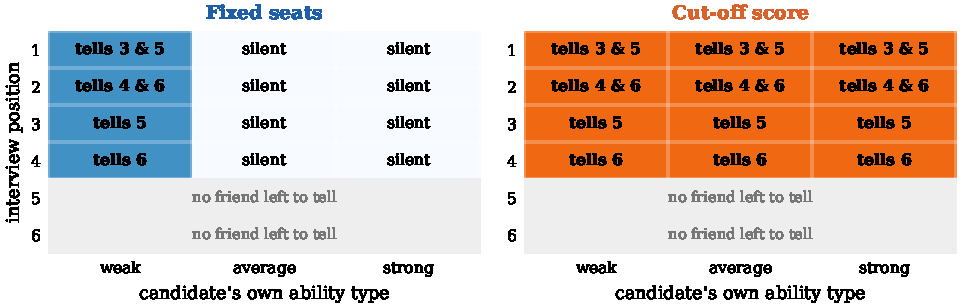
\includegraphics[width=\columnwidth]{figures/fig1_who_tells.pdf}
\caption{The equilibrium for two friend groups $\{1,3,5\}$, $\{2,4,6\}$ at $\alpha=0.2$ (E1). Under either rule it is the only pure equilibrium among 262{,}144 profiles.}\label{fig:who}
\end{figure}
\begin{table*}[t]\centering\small
\caption{Verification checks run before any experiment (\texttt{experiments/run\_checks.py}). ``Deviations'' are all rows of every type of every candidate, against both ``nobody shares'' and ``everybody shares''.}\label{tab:checks}
\resizebox{0.86\textwidth}{!}{\input{generated/tab_checks.tex}}
\end{table*}
\begin{figure*}[t]\centering
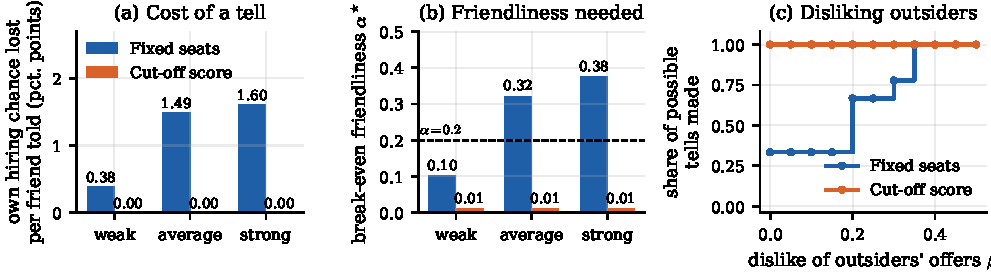
\includegraphics[width=0.86\textwidth]{figures/fig2_why_and_clans.pdf}
\caption{(a) Own hiring chance lost per friend told. (b) Break-even friendliness; types below the dashed line tell at $\alpha=0.2$. (c) Share of possible tells made in equilibrium as candidates
dislike outsiders' offers more ($\alpha=0.2$). Two friend groups, E1.}\label{fig:why}
\end{figure*}
Three stages: simulate the game into a table, solve the table (Level 1), let learners play the simulator (Level 2).
Unless a parameter is swept, $n=6$, $K=2$, $m=3$, $Q=15$, $\Delta=\sigma=1$, $c=0.001$.

\textbf{Stage 1: payoff tables.} For each of the $3^6=729$ type profiles $\theta$ and each of the $2^f$ sharing matrices ($f$ free entries; 64 for two friend groups)
we simulate 2{,}000 days and store $P(x_j=1\mid\theta,S)$, $P(x_ix_j=1\mid\theta,S)$ and $\E[V\mid\theta,S]$ for both rules. The same days are reused for every $S$ and both rules
(common random numbers), so payoff \emph{differences} --- all that equilibria depend on --- are precise, and Lemma~\ref{lem:mono} holds exactly in the table. All utilities are linear in the stored probabilities (\textsc{fair} uses the pairwise ones, $(x_j-x_i)^+=x_j-x_ix_j$),
so changing $\alpha$, $\beta$, $(a,b)$ or mixing utilities needs no new simulation. Means over 20 blocks of days are kept for the bootstrap.
Before any experiment the simulator reproduces the worked example and every structural result of Section~III (Table~\ref{tab:checks}), and 43 unit tests cover every module.

\textbf{Stage 2: solving the known game.} A pure strategy assigns one of $2^{|L(i)|}$ rows to each of three types: $4^3\cdot4^3\cdot2^3\cdot2^3=262{,}144$ profiles for two friend groups.
We precompute the \emph{interim value} $V_i[\sigma_{-i},\theta_i,a]=\E_{\theta_{-i}}[u_i(\theta,S(a,\sigma_{-i}(\theta_{-i})))]$ for every $\sigma_{-i}$; everything else is a lookup.
\begin{itemize}
\item \textbf{Pure equilibria, exhaustively:} keep every profile whose exploitability $\max_{i,\theta_i,a}V_i[\sigma_{-i},\theta_i,a]-V_i[\sigma_{-i},\theta_i,\sigma_i(\theta_i)]$ is 0; the list is complete.
Best-response dynamics from 8 starts must end in it; replicator dynamics on the 12 (candidate, type) agents looks for stable mixed equilibria.
\item \textbf{Mixed equilibria:} iterated strict dominance on every game; if every agent keeps one action, that profile is the only
equilibrium of any kind. On the pairs network (two actions per agent) we then enumerate the surviving supports and solve the indifference conditions.
\item \textbf{All CCEs at once:} two linear programs (HiGHS) per game maximise and minimise the expected share of tells over the CCE polytope. If they coincide, \emph{every} CCE --- every mixed or correlated equilibrium and every limit of no-regret play --- shares the same amount.
\item \textbf{Bootstrap $\varepsilon$:} resample the 20 blocks of days, rebuild the utilities and recompute the exploitability of the reported equilibrium; we report how often it stays exact and the 95th percentile of $\varepsilon$.
\item \textbf{Break-even friendliness:} $\alpha^\star=(\ell_i+c)/G_i$ from the table, and directly as the smallest $\alpha$ (grid step 0.025) at which the type tells in every equilibrium.
\end{itemize}
The complete network ($2^{15}$ matrices) is solved exhaustively at $n=4$; at $n=6$ we test ``nobody shares'' and ``everybody shares'' against every deviation of every type.

\begin{figure*}[t]\centering
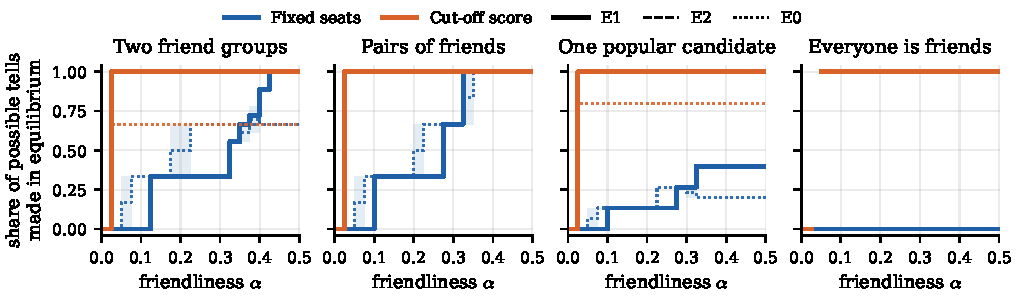
\includegraphics[width=0.95\textwidth]{figures/fig3_sharing_vs_friendliness.pdf}
\caption{Share of possible tells made in equilibrium as candidates care more about friends. Shaded bands: range over multiple equilibria (E0 only). ``Everyone is friends'' shows the profile
that passes the deviation test (E1).}\label{fig:alpha}
\end{figure*}
\textbf{Stage 3: learning the unknown game.} Each (candidate, type) is a bandit learner over that candidate's rows (12 learners with 4 or 2 arms). Each round draws fresh skills, the realised types'
learners choose, one day is simulated, and each learner sees only its own utility. Six learners: \textbf{$\varepsilon$-greedy} ($\varepsilon_t=t^{-1/3}$),
\textbf{UCB1}~\cite{ucb}, \textbf{Thompson sampling}~\cite{thompson}, \textbf{EXP3}~\cite{exp3}, and two of ours that also see how many of the told questions came up for each friend:
\begin{itemize}
\item \textbf{Leak-aware UCB} (Algorithm~\ref{alg:mb}): \emph{a tell matters only through questions that come up}. If none of my told questions appeared for my friend, the day went exactly as if I had not told her,
so the sample also counts for ``did not tell her''. In E1/E2 about half of all tells do not land ($0.8^3=0.51$); under E0 the learner is UCB1. In E1 the credit is exact; in E2 its bias is at most \EtwoBiasMax{} points (\EtwoBiasDays{} days), \EtwoBiasOverGap\% of the smallest payoff gap.
\item \textbf{Model-based UCB}: fits by ridge regression $r+c_n|a|=\mu_0+\sum_{j\in a}\beta_jk_j+\text{noise}$ ($k_j$: told questions that came up for friend $j$),
estimates the leak rate $\hat p$, and plays $\arg\max_a\mu_0+\sum_{j\in a}\beta_jm\hat p-c_n|a|$ plus a LinUCB bonus computed with an optimistic $\hat p$.
It is a reduced form of the review's learner: planning is single-agent, and the additive model cannot represent a redundant second tell (E0).
\end{itemize}

\begin{algorithm}[t]
\caption{One round of Leak-aware UCB for candidate $i$ of type $\theta$ (arms $a\subseteq L(i)$)}\label{alg:mb}
play $a=\arg\max_{a'}\ \hat\mu_{\theta,a'}+\sqrt{2\ln t_\theta/n_{\theta,a'}}$; observe own utility $r$ and, for each told friend $j\in a$, the number $k^{(i)}_j$ of told questions that came up\;
$D\leftarrow\{j\in a: k^{(i)}_j=0\}$ \tcp*{tells that did not land}
\For{every $a'$ with $a\setminus D\subseteq a'\subseteq a$}{
 $n_{\theta,a'}\mathrel{+}=1$; $\hat\mu_{\theta,a'}\leftarrow$ running mean with sample $r+c\,|a\setminus a'|$\;
}
$t_\theta\leftarrow t_\theta+1$\;
\end{algorithm}

\textbf{Measures.} \emph{Agreement}: share of the 12 learners whose currently-best arm is the equilibrium row. \emph{Regret}: Definition~3 with the table's expected payoffs.
\emph{CCE gap}: the largest average gain any candidate could have made by one fixed rule for the whole run. \emph{Rounds to 90\%}: first round with agreement $\ge0.9$.

\textbf{Experiments and statistics.} X1: rule $\times$ $\alpha\in\{0,0.025,\dots,0.5\}$ $\times$ four networks $\times$ E0--E2. X2: four utility families and five mixed populations.
X3: six learners $\times$ two rules $\times$ E0--E2, $T=\XthreeT$, \XthreeSeeds{} seeds. X4: bank size $Q\in\{4,\dots,64\}$ in E2, equilibrium re-solved for each $Q$ and $\alpha$. X5: $\Delta$, $\sigma$ or $K$ changed one at a time.
Runs that share a seed share every environment draw, so comparisons are paired: 95\% bootstrap CIs over seeds, sign-flip permutation tests, Holm correction~\cite{holm}.

% =====================================================================================================
\section{Results}\label{sec:results}

\subsection{Who tells? The hiring rule decides (RQ1)}\label{sec:who}
\begin{table*}[t]\centering\small
\caption{Equilibrium sharing for different motives (two friend groups A$=\{1,3,5\}$, B$=\{2,4,6\}$; E1). Every game has exactly one pure equilibrium.
$^\dagger$: exact equilibrium in fewer than 95\% of bootstrap replicates.}\label{tab:x2}
\resizebox{0.86\textwidth}{!}{\input{generated/tab_x2.tex}}
\end{table*}
\finding{Under fixed seats only weak candidates tell; under a cut-off everyone does} (Fig.~\ref{fig:who}): \PilotShareSeats\% against \PilotShareBar\% of the possible tells.
Under both rules the equilibrium is unique, every best-response and replicator run ends in it, and it stays exact in \PilotBootFracSeats\% / \PilotBootFracBar\% of \PilotBootRSeats{} bootstrap replicates.

\finding{Why: a weak candidate has almost nothing to lose} (Fig.~\ref{fig:why}a,b). Under fixed seats, telling one friend costs a weak candidate \EllSeatsWeak{} percentage points of her own
hiring chance, an average one \EllSeatsAvg{} and a strong one \EllSeatsStrong{}: a weak candidate is rarely at the last seat (with nobody sharing she holds it on \PivWeak\% of days, an average one on \PivAvg\%, a strong one on \PivStrong\%).
The friend gains about the same in all three cases (\GainSeatsWeak, \GainSeatsAvg, \GainSeatsStrong{} points), so $\alpha^\star=(\ell+c)/G$ is \AstarLocalSeatsWeak, \AstarLocalSeatsAvg{} and \AstarLocalSeatsStrong{}
(pilot: 0.09, 0.32, 0.37), and the exact equilibria switch at the next grid points (\AstarGridSeatsWeak, \AstarGridSeatsAvg, \AstarGridSeatsStrong). Under a cut-off the loss is exactly zero (Proposition~\ref{prop:bar}) and $\alpha^\star\approx\AstarLocalBarWeak$ for every type.

\finding{The staircase holds across networks and leak models} (Fig.~\ref{fig:alpha}; \XoneCells{} games). Under a cut-off, sharing jumps to its maximum at the first grid point above zero;
under fixed seats it climbs in steps --- weak, average, strong. A cut-off shares at least as much in \HtwoOk{} of \HtwoCells{} comparisons (strictly more in \HtwoStrict). Three details:
\begin{itemize}
\item \emph{The popular candidate never tells.} The star's hub has $\alpha^\star>1$ and is silent at every $\alpha\le0.5$ under fixed seats (Corollary~\ref{cor:hub}).
\item \emph{Everyone friends:} under fixed seats ``nobody shares'' passes the deviation test at all \CompGrid{} values of $\alpha$ (``everybody shares'' at \CompSeatsAllShare; Proposition~\ref{prop:clique} at $n=6$); under a cut-off ``everybody shares'' passes at \CompBarAllShare{} of the \CompGridPos{} values $\alpha>0$.
\item \emph{When told questions always come up (E0), a second tell is wasted,} so equilibria differ in \emph{who} tells. Only here are there several equilibria (\XoneMulti{} of \XoneCells{} games; the other \XoneUnique{} have exactly one),
and here is the one exception (\HtwoViolWhere): fixed seats have \HtwoViolSeatsN{} equilibria sharing \HtwoViolSeatsLo--\HtwoViolSeatsHi\%, the cut-off \HtwoViolBarN{} sharing \HtwoViolBar\%.
\end{itemize}
\begin{figure*}[t]\centering
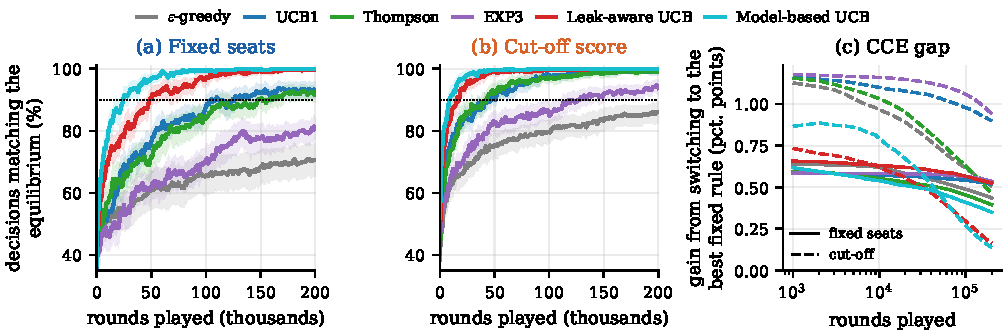
\includegraphics[width=0.9\textwidth]{figures/fig4_learning.pdf}
\caption{Learning in E1, mean over \XthreeSeeds{} seeds with 95\% bootstrap bands. (a,b) Share of the 12 (candidate, type) learners whose best arm is the equilibrium row.
(c) CCE gap of the history of play.}\label{fig:learn}
\end{figure*}
\begin{table*}[t]\centering\small
\caption{Decisions matching the equilibrium after \XthreeT{} rounds (\%, mean $\pm$ half-width of the 95\% CI over \XthreeSeeds{} seeds; best in bold), median rounds to reach 90\%
(``never ($x$\%)'': the median run did not, $x$\% of runs did), and cumulative regret after \XthreeT{} rounds (in units of one offer, mean over the 12 learners; lowest in bold).}\label{tab:x3}
\resizebox{0.9\textwidth}{!}{\input{generated/tab_x3.tex}}
\end{table*}
\finding{How solid are these equilibria?} The reported profile stays exact in at least 95\% of bootstrap replicates in \XoneBootOk{} of \XoneBootTot{} games; the exceptions sit on a step of the staircase,
and even there the 95th-percentile $\varepsilon$ is at most \XoneWorstEpsPP{} points: the \emph{pattern} is certain and each \emph{threshold} is known to within one grid step.
Best-response dynamics converged in \XoneBrdOk{} of \XoneBrdTot{} runs; replicator dynamics ended at an enumerated equilibrium in \XoneRepMatch{} of \XoneRepTot.


\finding{Mixed and correlated equilibria change nothing in E1 and E2, but widen E0.} Over \emph{all} CCEs, the maximum and minimum sharing coincide in \CceSingleEone{} of \CceTotEone{} (E1) and \CceSingleEtwo{} of \CceTotEtwo{} (E2) games:
no mixed or correlated equilibrium shares more or less than the pure one. In E0 the interval is wider than the pure range in \CceWiderEzero{} of \CceTotEzero{} games
(up to \CceEzeroAboveMax{} points above the largest pure sharing); only the pairs network, with one possible teller per friend, is untouched.
For two friend groups at $\alpha=0.2$ under a cut-off, the \CceExN{} pure equilibria share \CceExPure\%, correlated play \CceExLo--\CceExHi\%; \EzmRedundantBar\% of the extra tells go to a friend whom someone else already tells.
A second, independent implementation gives the same intervals in all \CceCrossRows{} rows.
Iterated strict dominance solves \DomSolved{} of the \DomTot{} games, each with a unique equilibrium of any kind; all but \DomOpenOutsideEzero{} of the rest are in E0.
On the pairs network, support enumeration finds one mixed equilibrium in each of the \SuppPairsMixedGames{} games left open, inside the CCE interval.

\subsection{What candidates care about (RQ2)}
\finding{Disliking outsiders makes candidates more generous to friends --- but only under fixed seats} (Fig.~\ref{fig:why}c). As $\beta$ rises from 0 to 0.5 at $\alpha=0.2$, sharing under
fixed seats rises from \ClanShareMinSeats\% to \ClanShareMaxSeats\% (everyone tells from $\beta=\ClanBetaFull$, i.e.\ $\alpha_{\text{eff}}=\ClanAlphaEffFull$, in line with the strong types' threshold), and stays at
\ClanShareMinBar\% under a cut-off, as the Remark of Section~III predicts.

\finding{Fairness-minded candidates behave the other way round} (Table~\ref{tab:x2}). Under fixed seats they never tell. Under a cut-off it is the \emph{strong} who tell, and only for moderate
inequality aversion: a strong candidate expects to be hired and dislikes being ahead of her friends; if envy ($a$) is large, the risk of being left behind dominates. This is the case Proposition~\ref{prop:bar} excludes.

\finding{Motives barely spill over.} In the \MixedGames{} mixed-population games, only \MixedDiffCells{} of \MixedCells{} (candidate, type) choices differs from what that candidate does in a population of her own kind.
In all \XtwoCceGames{} games of this section the CCE programs give a single sharing level, equal to the pure equilibrium's.

\subsection{Can candidates learn it? (RQ3)}\label{sec:learn}
\begin{figure*}[t]\centering
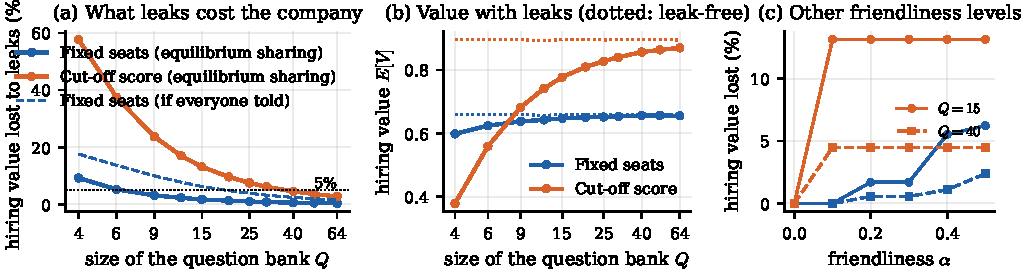
\includegraphics[width=0.9\textwidth]{figures/fig5_company_loss.pdf}
\caption{Company's hiring value under equilibrium sharing (E2, $m=3$). (a,b) As the question bank grows, $\alpha=0.2$; 95\% block-bootstrap intervals (\XfourBoot{} replicates) are narrower than the markers. (c) Loss against friendliness at $Q=15$ (solid) and $Q=40$ (dashed).}\label{fig:company}
\end{figure*}
\finding{Yes --- but the signal is tiny, so it takes tens of thousands of interviews.} At equilibrium the best row beats the second-best by only \PayGapMinEoneSeats--\PayGapMaxEoneSeats{} percentage points of utility under
fixed seats and \PayGapMinEoneBar--\PayGapMaxEoneBar{} under a cut-off, while a single outcome is 0 or 1. UCB1 and Thompson sampling still end with \AgreeUcbEoneSeats\% and \AgreeTsEoneSeats\% (seats)
and \AgreeUcbEoneBar\% and \AgreeTsEoneBar\% (cut-off) of decisions correct in E1 (Table~\ref{tab:x3}); EXP3 and $\varepsilon$-greedy are slower. E2 is the same within error bars.

\finding{Finding the equilibrium and earning along the way are different things.} Regret ranks the learners almost the other way round: under fixed seats in E1 it is \RegretEpsEoneSeats{} for $\varepsilon$-greedy and
\RegretTsEoneSeats{} for Thompson sampling against \RegretUcbEoneSeats{} for UCB1. With gaps this small UCB1's bonus never lets it settle: it ends with the right most-played row but puts \ExpWrongUcbSeats\% of its pulls (seats) on other rows ($\varepsilon$-greedy: \ExpWrongEpsSeats\%).

\finding{A cut-off is easier to learn} whenever the equilibrium is unique: the gap is larger and the same for all types; agreement under a cut-off is significantly higher in \BarSeatsSig{} of \BarSeatsTests{} paired E1/E2 tests (the rest are at 100\% under both).
Under fixed seats the \emph{average} types are learned slowest (UCB1: \TypeUcbEoneSeatsWeak, \TypeUcbEoneSeatsAvg{} and \TypeUcbEoneSeatsStrong\% correct for weak, average, strong): their reward noise relative to their payoff gap is largest
(squared noise over squared gap \ExpSnrWeak, \ExpSnrAvg, \ExpSnrStrong; rank correlation with the final error rate $\rho=\ExpRhoUcb$ for UCB1).

\begin{figure*}[t]\centering
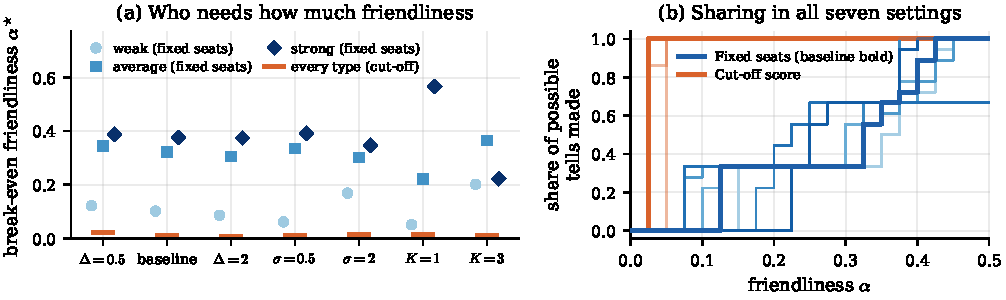
\includegraphics[width=0.8\textwidth]{figures/fig6_sensitivity.pdf}
\caption{Two-groups game (E1) with one parameter moved at a time. (a) Break-even friendliness by type under fixed seats, and the single value of every type under a cut-off. (b) Equilibrium sharing in all seven settings; baseline bold.}\label{fig:sens}
\end{figure*}
\finding{Knowing how leaks work is worth a factor of two to five.} In E1, 90\% agreement takes Leak-aware UCB \TninetyMbEoneSeats{} rounds under fixed seats and \TninetyMbEoneBar{} under a cut-off, Model-based UCB \TninetyMuEoneSeats{} and \TninetyMuEoneBar,
UCB1 \TninetyUcbEoneSeats{} and \TninetyUcbEoneBar; both leak-using learners end at 100\% in E1 and E2, and at 20{,}000 rounds lead UCB1 significantly in all E1/E2 settings.
Leak-aware UCB lowers regret mainly under a cut-off ($\MbRegretEoneBar$), where the best arm ``tell everyone'' informs every other arm. Model-based UCB lowers regret in all four E1/E2 settings ($\MuRegretEoneSeats$ and $\MuRegretEoneBar$ in E1)
and its leak-rate estimate is right ($\hat p=\MuLeakHatEone$, truth $0.2$).

\finding{Play moves toward the CCE set, but is not yet close to it} (Fig.~\ref{fig:learn}c). Between 10{,}000 and \XthreeT{} rounds the CCE gap falls for all six learners
(significant in \GapFallSetSig{} of \GapFallSetTests{} learner-by-setting tests) but ends at \GapFinalMin--\GapFinalMax{} points --- about the size of the payoff gaps, so exploration is still being paid for.
No learner's settled profile is below random sharing in welfare (\BaseLearnBelowWelfare{} exceptions in 24 comparisons).

\finding{A caution about ``agreement'' in E0.} In E0 with a cut-off agreement looks poor (\AgreeEzeroBarMin--\AgreeEzeroBarMax\%): the \NumEqEzeroBar{} equilibria differ only in which of two friends tells the last
candidate, and the learners end up both telling. The settled profile is an exact equilibrium in \ExactEzeroBarMax\% of these runs but within one
message cost of one in \WithinCEzeroBarMin\%: \LcSettledHighN{} of the \LcSettledN{} learners settle on profiles sharing \LcSettledHighShareMin--\LcSettledHighShareMax\%, at or just above the top of the CCE interval (\CceExLo--\CceExHi\%) --- the redundant telling of Section~\ref{sec:who}.

\subsection{What it costs the company (RQ4)}\label{sec:cost}
\begin{table*}[t]\centering\footnotesize
\caption{The five hypotheses fixed in the project review, the refutation criterion fixed with them, and what the experiments say.}\label{tab:hyp}
\begin{tabular}{@{}p{0.4cm}>{\raggedright\arraybackslash}p{3.7cm}>{\raggedright\arraybackslash}p{2.9cm}>{\raggedright\arraybackslash}p{7.3cm}>{\raggedright\arraybackslash}p{2.0cm}@{}}
\toprule
 & Hypothesis & Refuted if (review) & Evidence & Verdict\\\midrule
H1 & Under fixed seats, $\alpha^\star$ is highest for the types most likely to be pivotal & $\alpha^\star$ flat, or lowest for pivotal types &
$\alpha^\star=\AstarLocalSeatsWeak<\AstarLocalSeatsAvg<\AstarLocalSeatsStrong$, the order of how often a type holds the last seat with nobody sharing (\PivWeak, \PivAvg, \PivStrong\%); at $K=1,2,3$ the two orders match (at $K=3$ average types are the pivotal ones) & Supported\\
H2 & Cut-off shares more than fixed seats for every $\alpha\in[0,0.5]$ & Fixed seats share more at some $\alpha$ &
Holds in all \HtwoCellsNoEzero{} E1/E2 comparisons. In E0 fails once (\HtwoViolWhere): fixed seats have equilibria sharing up to \HtwoViolSeatsHi\%, the cut-off \HtwoViolBar\% &
Refuted once (E0); holds in E1/E2\\
H3 & Fixed seats: sharing rises with $\beta$; cut-off: no effect & No rise under fixed seats, or an effect under a cut-off & \ClanShareMinSeats\%$\to$\ClanShareMaxSeats\% (never falling) vs.\ constant \ClanShareMinBar\% & Supported\\
H4 & No-regret play nears the CCE set; model-based learners are faster & CCE gap does not fall, or not faster &
CCE gap falls significantly in \GapFallSetSig{} of \GapFallSetTests{} tests but ends at \GapFinalMin--\GapFinalMax{} points, the size of the payoff gaps; Model-based UCB reaches 90\% in \TninetyMuEoneSeats/\TninetyMuEoneBar{} rounds (leak-aware UCB: \TninetyMbEoneSeats/\TninetyMbEoneBar) vs.\ \TninetyUcbEoneSeats/\TninetyUcbEoneBar{} for UCB1 & Faster: supported; nears the CCE set: weak\\
H5 & $\Lambda_{\textsc{bar}}>\Lambda_{\textsc{seats}}$, and fixed seats need a smaller $Q$ for $\Lambda<5\%$ & CI includes 0, or order reversed &
At $\alpha=0.2$: \LamRatioMin--\LamRatioMax$\times$ larger, disjoint CIs at every $Q$; $Q\ge\QFiveSeats$ vs.\ $Q\ge\QFiveBar$; larger at every $\alpha>0$ and $Q$ (\XfourRobBarMore{} of \XfourRobPairs) & Supported\\
\bottomrule
\end{tabular}
\end{table*}
\finding{At $\alpha=0.2$, leaks hurt a cut-off company about ten times more --- mostly because more people tell.} With a bank of 15 questions, equilibrium sharing costs \LamSeatsQFifteen\% of hiring value under fixed seats and \LamBarQFifteen\% under a cut-off;
across all bank sizes the cut-off loses \LamRatioMin--\LamRatioMax{} times more, with disjoint bootstrap intervals at all \LamOrderTot{} sizes (Fig.~\ref{fig:company}a). Keeping the loss below 5\% needs $Q\ge\QFiveSeats$ under fixed seats and $Q\ge\QFiveBar$ under a cut-off
(Proposition~\ref{prop:leak}: the leaked fraction falls like $m\,n_j/Q$). Two effects add up: \emph{who} tells (\XfourShareBar\% of possible tells under a cut-off, \XfourShareSeats\% under fixed seats), and the rule:
every leaked mark can lift someone over a fixed line, whereas under fixed seats a leak only reorders candidates. If everyone told under both rules (dashed line), the cut-off would lose only \LamAllRatioMin--\LamAllRatioMax{} times more.

\finding{The order holds at every friendliness} (Fig.~\ref{fig:company}c): re-solving every bank size for $\alpha\in\{0,0.1,\dots,0.5\}$, the cut-off loses more in all \XfourRobBarMore{} games with $\alpha>0$;
the ratio is \XfourRobRatioLowMin--\XfourRobRatioLowMax$\times$ at $\alpha=0.2$--$0.3$ and \XfourRobRatioHighMin--\XfourRobRatioHighMax$\times$ at $\alpha\ge0.4$, as more types tell under fixed seats.

\finding{But the cut-off is still the better rule once the bank is large enough} (Fig.~\ref{fig:company}b). Without leaks a cut-off hires better (\VNoLeakBar{} against \VNoLeakSeats): it can hire three good candidates or none,
where fixed seats must hire two. Leaks eat this advantage only for small banks: fixed seats give more value up to $Q=\CrossQBarWorseUpTo$, the cut-off from $Q=\CrossQBarBetterFrom$.
With a cheaper charge per hire than $\tau_K$ ($\kappa=0$ or $\tau_K/2$), the cut-off is better at every bank size. For a company the message is not ``avoid cut-offs'' but ``a cut-off needs a larger bank''.

\subsection{How robust is the staircase? (X5)}
The bootstrap measures only Monte Carlo error, so we re-solved the headline game exactly in \XfiveSettings{} settings ($\Delta\in\{0.5,1,2\}$, $\sigma\in\{0.5,1,2\}$, $K\in\{1,2,3\}$, one at a time; \XfiveGames{} games; Fig.~\ref{fig:sens}).
\finding{The mechanism survives everywhere; the exact order of the types does not.} In all \XfiveSettings{} settings a tell costs nothing under a cut-off,
the cut-off shares at least as much as fixed seats (\XfiveHtwoCellsOk{} of \XfiveHtwoCells{} comparisons), and under fixed seats $\alpha^\star$ ranks the types exactly as their own loss $\ell$
does. Weak $<$ average $<$ strong holds in \XfiveOrderOk{} of them. The exception is $K=3$: the marginal seat sits at the
median, a tell costs an \emph{average} candidate most (\XfiveKthreeEllWeak, \XfiveKthreeEllAvg, \XfiveKthreeEllStrong{} points per friend told) and the thresholds follow
(\XfiveKthreeWeak, \XfiveKthreeAvg, \XfiveKthreeStrong). With nobody sharing, at $K=3$ an average candidate holds the last seat on \PivKthreeAvg\% of days, a strong one on \PivKthreeStrong\%, a weak one on \PivKthreeWeak\%:
for every $K$ the type most often at the margin needs the most friendliness. With $K=1$ a strong candidate needs $\alpha^\star=\XfiveKoneStrong$ and never tells on our grid.

\subsection{Verdict on the hypotheses, deviations and limits}
Judged by the criteria fixed in the review (Table~\ref{tab:hyp}), H1, H3 and H5 are supported. H4 is not refuted, with unequal support: the faster-learner half holds clearly, but the CCE gap falls without becoming small.
H2 is refuted at one point in E0, where the game has several equilibria; in E1 and E2 it holds in every comparison.
\textbf{Deviations from the review plan:} (i)~2{,}000 days per cell, not 8{,}000, with precision reported per equilibrium by the bootstrap; (ii)~the ``model-based'' learner is built in two simpler forms (Section~\ref{sec:method});
(iii)~support enumeration on the pairs network only, with the CCE programs bounding the rest; (iv)~the complete network at $n=6$ was handled by deviation tests, and $n=8$ was not attempted.
\textbf{Limits.} Types are coarse and rounds independent: no reputation, and placed candidates do not leave the pool (a stochastic game~\cite{shapley}). Networks are fixed and small, there is no real leak data, so every claim is comparative,
and sensitivity was tested one parameter at a time for one network.

% =====================================================================================================
\section{Contribution}
{\centering\footnotesize
\begin{tabular}{@{}>{\raggedright\arraybackslash}p{1.25cm}>{\raggedright\arraybackslash}p{4.85cm}>{\raggedright\arraybackslash}p{1.6cm}@{}}
\toprule
Member & Task assigned in the review; where it is delivered & Status\\\midrule
Jash Bharat Pasad & Formulation, proofs; utility types (X2); company analysis (X4); writing. Sections II--III; \texttt{utility.py}, \texttt{run\_x2.py}, \texttt{run\_x4.py}; Table~\ref{tab:x2}, Fig.~\ref{fig:company} & Fulfilled\\
Bhavay Goyal & Simulator (E0--E2, networks), payoff tables, verification checks, pipeline. \texttt{config.py}, \texttt{env.py}, \texttt{tables.py}, \texttt{checks.py}, unit tests; also X5 (\texttt{run\_sensitivity.py}, Fig.~\ref{fig:sens}) and an independent CCE implementation & Fulfilled; plus X5 and CCE cross-check\\
Chaitanya Bhoite & Level-1 solvers (BNE, mixed equilibria, CCE program, bootstrap); X1. \texttt{game.py}, \texttt{solvers.py}, \texttt{support\_enum.py}, \texttt{run\_x1.py}, \texttt{run\_cce.py}; Figs.~\ref{fig:who}--\ref{fig:alpha} & Fulfilled; support enumeration on pairs only\\
Vishnu Sinha & Level-2 learners (incl.\ model-based); regret and CCE metrics; X3; statistics. \texttt{learners.py}, \texttt{learning.py}, \texttt{stats.py}, \texttt{run\_x3.py}; Fig.~\ref{fig:learn}, Table~\ref{tab:x3} & Fulfilled; model-based learner in reduced form\\
\bottomrule
\end{tabular}\par}
\smallskip
Core (verified simulator, X1--X3, H1--H4) and target (X4, H5) deliverables are complete; the stretch target $n=8$ is not.
Every number in this report is generated from the result files in the repository by \texttt{experiments/make\_figures.py}; the README lists the command behind each figure and table.

\begin{thebibliography}{15}\footnotesize\setlength{\itemsep}{0pt}
\bibitem{blind} Team Blind, ``Candidate confessed to memorizing leaked interview questions,'' \url{https://www.teamblind.com}, accessed Sept.\ 2026.
\bibitem{glider} Glider AI, ``Leaked interview questions: How candidates get answers,'' \url{https://glider.ai}, accessed Sept.\ 2026.
\bibitem{lazear} E.~P. Lazear and S. Rosen, ``Rank-order tournaments as optimum labor contracts,'' \emph{J. Polit. Econ.}, vol.~89, no.~5, pp.~841--864, 1981.
\bibitem{krakel} M. Kr\"akel, ``Helping and sabotaging in tournaments,'' \emph{Int. Game Theory Rev.}, vol.~7, no.~2, pp.~211--228, 2005.
\bibitem{li} Y. Li and V. Conitzer, ``Game-theoretic question selection for tests,'' \emph{J. Artif. Intell. Res.}, vol.~59, pp.~437--462, 2017.
\bibitem{ucb} P. Auer, N. Cesa-Bianchi, and P. Fischer, ``Finite-time analysis of the multiarmed bandit problem,'' \emph{Mach. Learn.}, vol.~47, pp.~235--256, 2002.
\bibitem{exp3} P. Auer, N. Cesa-Bianchi, Y. Freund, and R.~E. Schapire, ``The nonstochastic multiarmed bandit problem,'' \emph{SIAM J. Comput.}, vol.~32, no.~1, pp.~48--77, 2002.
\bibitem{thompson} W.~R. Thompson, ``On the likelihood that one unknown probability exceeds another in view of the evidence of two samples,'' \emph{Biometrika}, vol.~25, pp.~285--294, 1933.
\bibitem{hart} S. Hart and A. Mas-Colell, ``A simple adaptive procedure leading to correlated equilibrium,'' \emph{Econometrica}, vol.~68, no.~5, pp.~1127--1150, 2000.
\bibitem{wellman} M.~P. Wellman, ``Methods for empirical game-theoretic analysis,'' in \emph{Proc. AAAI}, 2006, pp.~1552--1556.
\bibitem{shoham} Y. Shoham and K. Leyton-Brown, \emph{Multiagent Systems: Algorithmic, Game-Theoretic, and Logical Foundations}. Cambridge Univ. Press, 2008.
\bibitem{fehr} E. Fehr and K.~M. Schmidt, ``A theory of fairness, competition, and cooperation,'' \emph{Q. J. Econ.}, vol.~114, no.~3, pp.~817--868, 1999.
\bibitem{holm} S. Holm, ``A simple sequentially rejective multiple test procedure,'' \emph{Scand. J. Stat.}, vol.~6, no.~2, pp.~65--70, 1979.
\bibitem{shapley} L.~S. Shapley, ``Stochastic games,'' \emph{Proc. Natl. Acad. Sci.}, vol.~39, no.~10, pp.~1095--1100, 1953.
\end{thebibliography}
\end{document}
